% What Does a Fly's Wiring Know? A Fruit-Fly Brain in Minecraft
% Preprint (27 Sep 2026). Build: ./build.sh (flycraft.tex is put together by assemble.py from this preamble,
% flycraft_main.tex, flycraft_notes.tex and references_pool.tex).
% Every number traces to a result file: ../experiments/results/ (re-run 26-27 Sep 2026, identical to the digit to the
% run before) and ../experiments/results_edge/ (the edge-case suite; RESEARCH_NOTES 23, experiments/edge/analysis_*.md).
% Build: ./build.sh

\documentclass[11pt,a4paper]{article}

\usepackage[utf8]{inputenc}
\usepackage[T1]{fontenc}
\usepackage{lmodern}
\usepackage[margin=1in]{geometry}
\usepackage{amsmath,amssymb}
\usepackage{booktabs}
\usepackage{graphicx}
\usepackage{xcolor}
\usepackage{hyperref}
\usepackage{cleveref}
\usepackage{enumitem}
\usepackage{natbib}
\usepackage{url}
\usepackage{microtype}
\usepackage{caption}
\usepackage{array}
\usepackage{tabularx}
\usepackage{ragged2e}
\usepackage{tikz}
\usetikzlibrary{positioning,arrows.meta,calc}

\hypersetup{colorlinks=true, linkcolor=blue!60!black, citecolor=blue!60!black, urlcolor=blue!60!black}
\bibpunct{(}{)}{;}{a}{,}{,}
\captionsetup{font=small,labelfont=bf}
\crefname{figure}{Figure}{Figures}
\crefname{table}{Table}{Tables}
\crefname{section}{Section}{Sections}
\setlength{\emergencystretch}{3em}
\urlstyle{same}
\renewcommand{\topfraction}{0.9}
\renewcommand{\textfraction}{0.07}
\renewcommand{\floatpagefraction}{0.75}
\newcommand{\note}[1]{(Note~#1)}

\title{%
  \textbf{What Does a Fly's Wiring Know?\\
  A Fruit-Fly Brain in Minecraft}%
}
\author{
  Solomon Shalom Lijo \\
  Independent Researcher \\
  \texttt{solomon@getromy.app}
}
\date{September 27, 2026}

\begin{document}
\maketitle

\begin{abstract}
\noindent I ask what the complete wiring diagram of a fruit fly's brain knows about meeting another fly. To find out, I run a published simulation of that diagram as the brain of a fly in Minecraft, first on its own, then with one internal state switched on, then with a learning rule. I try hard to break every result. Run this way, I argue, the wiring knows how to react but not what it wants. The senses send mostly ``no'' or nothing to the neurons that decide whether to accept a male or fight, but keeping the female's two ``virgin'' neurons firing wakes her acceptance neurons. Keeping hunger neurons firing does no more than keeping an unrelated group firing. A memory forms once I supply the teaching signal that the model's taste neurons fail to send, and the fly hardly ever uses it. Along the way I found that most smells leave the model firing on its own for as long as I watched, and that several things I first believed were wrong.
\end{abstract}

\medskip
\noindent\textbf{Keywords:} connectome, \emph{Drosophila}, whole-brain simulation, innate behaviour, courtship, Minecraft

% ══════════════════════════════════════════════════════════════════════════════
\section{Introduction}
\label{sec:introduction}

Fruit-fly geneticists name a gene after what goes wrong when it breaks. A fly with a broken \emph{dunce} gene cannot learn that a smell comes with an electric shock \citep{dudai1976dunce}. A male with a broken \emph{fruitless} gene courts other males \citep{ryner1996control}. Behind the jokey names is the idea that much of what a fly does comes built in. Reared alone, a male courts the first virgin female he meets, and does it properly \citep{siegel1979conditioned}. He follows her, taps her with a foreleg to taste her, stretches out one wing and vibrates it to sing, and tries to mate. She decides. A virgin slows down and lets him. A female who has mated recently walks off, kicks, and holds out her ovipositor, the tube at the tip of her abdomen that she lays eggs through, until he gives up \citep{greenspan2000courtship}.

But built into what? A behaviour that nobody taught could live in two quite different places. It could be in the wiring, in which neuron connects to which, the way the ring of a doorbell lives in the circuit between the button and the bell. Or it could need the fly to be in a particular state, virgin or mated, hungry or fed. And some social behaviour is learned: a male who has spent an hour being turned down by a mated female courts half-heartedly for hours afterwards \citep{siegel1979conditioned}. In a living fly the three cannot be pulled apart, because every fly that has wiring also has states and a past.

A simulation can pull them apart. In 2024 the FlyWire consortium published the wiring diagram of a whole female fly brain, 139{,}255 neurons and about fifty million synapses \citep{dorkenwald2024neuronal}. A male followed in September 2026, with the nerve cord that runs his legs and wings \citep{berg2026sexual}. \citet{shiu2024drosophila} had already turned the female diagram into a simulation with one model neuron for every real one, and found that it does some of what flies do. A simulation like that is a fly with wiring and nothing else. It has no hormones or moods, and it has never learned anything. Whatever it does, the wiring can do alone. Whatever it cannot do needs something else, and I can add the something else back one piece at a time.

Forty years after the first complete wiring diagram, of a worm with 302 neurons \citep{white1986structure}, biologists still argue about how much of the worm's behaviour it explains. Much of the worm runs on chemistry, which a diagram does not show \citep{bargmann2013connectome}. Diagrams of bigger brains now cost a great deal \citep{microns2025functional}, so it is worth asking what a complete one knows on its own.

So I gave the simulated brain a body in Minecraft (\Cref{fig:overview}) and put two flies in a box.

\subsection{The Argument in Brief}
\label{sec:brief}

\emph{First}, the wiring alone carries reflexes. The simulated fly works her mouthparts on sugar and extends her ovipositor when her head is touched, and a randomly rewired brain does neither. \emph{Second}, it carries none of the decisions. The neurons with which a female accepts a male or fights another female can fire, but the senses tell them no, or nothing. A few of the male's courtship neurons do fire, mostly to the smell of another male. \emph{Third}, keeping her two ``virgin'' neurons firing wakes her acceptance neurons. Keeping the hunger and fullness neurons firing does no more than keeping an unrelated group firing, and real flies carry those states mostly in chemicals. \emph{Fourth}, once I supply the teaching signal that taste fails to deliver, the fly learns which smell came with sugar and does nothing with it. \emph{Fifth}, two flies in a box do not steer towards each other. So in this model ``built in or learned?'' has at least four answers: wiring, states carried by wires, states carried by chemicals, and learning. The diagram carries the first two, once someone switches the state on.

\subsection{Contributions}

I make four contributions.

\begin{enumerate}[leftmargin=*]
  \item A body in Minecraft for the published whole-brain fly model, and a male brain built the same way (\Cref{sec:experiment}).
  \item A map of which social behaviours this model produces from wiring alone, which need one internal state and which it cannot produce (\Cref{sec:reflexes,sec:absent,sec:states,sec:memory,sec:arena}).
  \item Two findings about the model itself. Its published smell centre cannot tell smells apart (\Cref{sec:experiment}), and most smells leave the model firing on its own after they have gone (\Cref{sec:absent}).
  \item A record of trying to break all of this, which overturned several of my own first claims (\Cref{sec:breaking}).
\end{enumerate}

\subsection{What This Paper Is Not}

It is not a claim that the model is a fly. A wiring diagram is to a brain roughly what a road map is to traffic: it shows every road and junction, but not which roads are busy or where anyone wants to go. The model adds some of the simplest traffic rules anyone has proposed, so when the simulated fly fails, the fault may lie in those rules, and I try to say when. Nor is it a new brain model. I rebuilt Shiu et al.'s and changed two things, both reversible (\Cref{sec:experiment}). Everything here happens in a computer, and testing its predictions (\Cref{sec:refutation}) is work for people with flies.

\subsection{Author Position}

I am an independent researcher. My earlier papers are about evaluating AI systems \citep{lijo2026compound,lijo2026pifbench,lijo2026niche,lijo2026tsb,lijo2026spirits}, and I have no training in biology. This paper does the same job on a different system: it puts a published model through tests, most with pass marks fixed in advance, and reports where it fails. An AI coding assistant helped to write the simulator, the Minecraft body, the analysis scripts and drafts of this text. Other copies of it then checked the claims against the result files (\Cref{sec:breaking}). Those copies share its blind spots, and nobody outside the project has checked the work yet.

This paper reads differently from my others because, unlike them, it was fun to do. I wanted to see what a fly's brain would do if I let it loose in Minecraft. So I have written it the way I would tell it, in the manner of Bill Capra's \emph{The Metaphysics of Farts} \citep{capra2022metaphysics}, a short essay that treats a silly subject with a straight face. The tests are as strict as in my other papers.

\subsection{Roadmap}

\Cref{sec:guide} is a guide for readers without biology and \Cref{sec:experiment} describes the experiment. \Cref{sec:reflexes,sec:absent,sec:states,sec:memory,sec:arena} give the results, \Cref{sec:breaking} tries to break them, and the last sections answer objections and list what would prove me wrong. The numbered notes hold the numbers. The story does not need them.

% ══════════════════════════════════════════════════════════════════════════════
\section{A Fly Brain for Readers Without Biology}
\label{sec:guide}

Nothing in the main text needs more biology than this section.

\subsection*{Neurons and spikes}

A neuron is a cell that passes on messages as tiny electrical pulses called spikes. How busy a neuron is gets counted in spikes per second, written Hz. A neuron at rest fires 0\,Hz, a busy one 50 or 100. To \emph{drive} a neuron is to make it fire. Where one neuron meets the next there is a synapse. A spike arriving at an excitatory synapse nudges the next neuron towards firing, and one arriving at an inhibitory synapse nudges it away. Which kind a neuron makes depends mostly on the chemical it releases, its neurotransmitter. For most neurons nobody has measured that chemical. The model uses a guess made by a computer program (a classifier) from microscope pictures, and makes each neuron all ``go'' or all ``stop''. That is the neuron's sign. Some neurons also pass current through direct contacts, called electrical synapses. The model has none.

\subsection*{The wiring diagram}

A fruit fly's brain has about 140{,}000 neurons (a human brain has about 600{,}000 times as many). A wiring diagram, or connectome, lists which neuron connects to which, and through how many synapses. It records nothing about what travels along the wires.

\subsection*{Three kinds of neuron}

Sensory neurons turn the world into spikes: smell receptors on the antennae, taste neurons on the mouthparts and legs, bristles that fire when they are bent, and an ear in the antenna. Descending neurons, about 1{,}300 of them, carry commands down the neck to the legs and wings. Everything in between, over a hundred thousand neurons, is where any deciding has to happen. \Cref{tab:cast} lists the neurons this paper mentions and the names I use for them.

\subsection*{States and chemistry}

A fly can be hungry or fed, virgin or mated. Part of that is carried by particular neurons that keep firing steadily. The virgin neurons, for example, fire until the female mates. Part is carried by chemicals such as hormones and neuropeptides (small protein messengers), released into the brain to change how other neurons respond. Biologists call this neuromodulation \citep{marder2012neuromodulation}. A wiring diagram can show the first kind but not the second.

\subsection*{Learning}

A fly learns which smells go with food in a part of its brain called the mushroom body. A smell switches on a small set of its cells, and if a dopamine ``teacher'' neuron fires at the same moment, the connections from those cells to the mushroom body's output neurons weaken. The next time the smell arrives, the output neurons hear it more faintly. That weakening is the memory. The output neurons push the fly towards or away from things.

\subsection*{Three technical words}

A \emph{seed} fixes the program's random numbers, such as when each stimulated neuron fires. Running several seeds is like testing the same fly again with fresh luck, so it shows how much a number wobbles by chance. The \emph{gain} turns every synapse in the brain up or down together. A gain of 1 is the published strength, and 1.4 makes each synapse 40 per cent stronger. A result that appears at only one exact gain is a coincidence of the numbers. A \emph{rewired} brain is the same brain with its connections shuffled at random, each neuron keeping its number of connections. A behaviour that survives rewiring cannot be due to the particular wiring alone.

\begin{table}[tbp]
\centering
\small
\renewcommand{\arraystretch}{1.1}
\begin{tabularx}{\textwidth}{@{}>{\RaggedRight}p{3.3cm}>{\RaggedRight}p{3.2cm}>{\RaggedRight\arraybackslash}X@{}}
\toprule
\textbf{Neurons} & \textbf{Nickname here} & \textbf{What they do in a real fly} \\
\midrule
MN9 & the licking neuron & swings the mouthparts out to feed \citep{shiu2024drosophila} \\
Giant fibre (DNp01) & the escape neuron & fires the escape jump \citep{vonreyn2014spike} \\
aBN1 & the grooming neuron & starts antennal grooming \citep{hampel2015neural} \\
DNa01, DNa02 & the steering neurons & turn a walking fly left or right \citep{rayshubskiy2025neural} \\
MDN & the moonwalker & walks the fly backwards \citep{bidaye2014neuronal} \\
DNp13 & the ovipositor neuron & extends the ovipositor, which a virgin does to accept a male and a mated female to refuse one \citep{mezzera2020ovipositor} \\
Or67d neurons & the pheromone detector & smell cVA, a scent males make that other flies react to \citep{kurtovic2007single} \\
SAG & the virgin neurons & active in virgins, turned down by mating \citep{feng2014ascending} \\
pC1a--c; pC1d/e, aIPg & the female's deciders: acceptance neurons; aggression deciders & set how receptive, or how aggressive, she is \citep{wang2021neural,deutsch2020neural,schretter2020cell} \\
vpoEN & the song relay & carry the male's song to the yes neuron \citep{wang2021neural} \\
vpoDN (DNp37) & the yes neuron & opens the genital plate to accept a male \citep{wang2021neural} \\
oviDN & the egg-laying neurons & start egg-laying \citep{wang2020neural} \\
P1; pIP10 & courtship neurons (his deciders); song command & start a male's courtship; send his song command to the wing \citep{vonphilipsborn2011neuronal,kohatsu2011female} \\
IPC (insulin), DH44, NPF, SIFa, AstA & hunger and fullness neurons & signal whether the fly has fed, largely by releasing neuropeptides \citep{pool2014feeding} \\
PAM, PPL1; MBONs & the teachers; the memory's outputs & reward and punishment signals to the mushroom body; its output neurons \citep{aso2014neuronal} \\
\bottomrule
\end{tabularx}
\caption{The cast: the neurons that appear in this paper, the nicknames I use for them, and what experiments on real flies have found them to do.}
\label{tab:cast}
\end{table}

% ══════════════════════════════════════════════════════════════════════════════
\section{The Experiment}
\label{sec:experiment}

Shiu et al.'s model treats every neuron as a leaky bucket. Each spike from a neighbour pours in a fixed cupful for every synapse between them, or scoops one out if the neighbour is inhibitory. The bucket leaks, and when the water rises 7 millivolts above its resting level it overflows: the neuron fires and empties. Nothing is tuned to make the fly behave. At full numerical precision my rebuild matches a transcription of their code spike for spike. At the lower precision I use for speed, a neuron on the brink of overflowing can tip the other way. In one of three test runs the difference then spreads to about a fifth of the spikes, though their total changes by under 1 per cent \note{1}.

Twenty times a second the Minecraft body turns what the fly smells, tastes and touches into firing of its own sensory neurons, and its own descending neurons move the body (\Cref{fig:overview}). Flowers smell of fruit or vinegar. Another fly smells of fly, and a male also of cVA, his pheromone, a scent one fly makes to signal to others. Bumping into anything fires every bristle on the head. The female map stops at the neck, so she walks on her steering neurons: the harder they fire the faster she goes, and when one side fires harder she turns that way. Nothing in the body says ``if touched, back away''. If the fly backs away, its moonwalker neurons fired. The flies are in effect blind. Light makes their eyes fire, but the eye's first relay neurons signal partly by being turned down, which a model neuron at rest cannot pass on. I built a male brain the same way from the male map.

Most of the numbers come from the bench, without Minecraft. I make one set of sensory neurons fire, usually 100 times a second for a second, and count what fires elsewhere. A louder sound or a harder touch means a higher rate.

\begin{figure}[tbp]
\centering
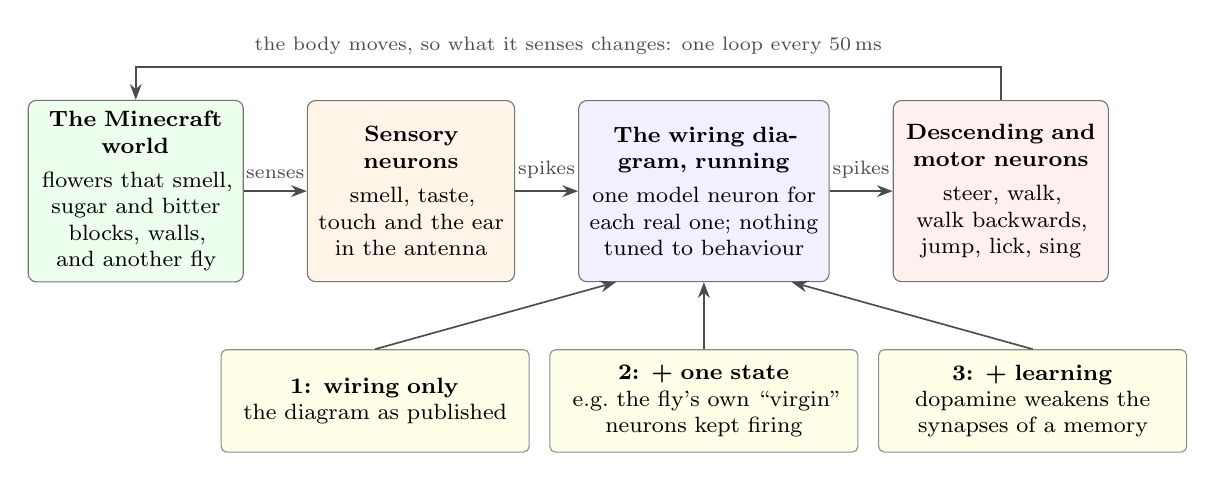
\begin{tikzpicture}[
  font=\footnotesize,
  box/.style={draw=black!55, rounded corners=3pt, align=center, inner sep=4pt, minimum height=2.3cm, text width=#1},
  arr/.style={-{Stealth[length=2mm]}, semithick, black!70},
  lab/.style={font=\scriptsize, text=black!70, above=1pt},
  sw/.style={draw=black!45, rounded corners=2pt, align=center, inner sep=3pt, text width=3.7cm, minimum height=1.3cm, fill=yellow!9},
]
\node[box=2.45cm, fill=green!7] (world) {\textbf{The Minecraft world}\\[3pt] flowers that smell, sugar and bitter blocks, walls, and another fly};
\node[box=2.35cm, fill=orange!9, right=0.8cm of world] (sense) {\textbf{Sensory neurons}\\[3pt] smell, taste, touch and the ear in the antenna};
\node[box=2.9cm, fill=blue!6, right=0.8cm of sense] (brain) {\textbf{The wiring diagram, running}\\[3pt] one model neuron for each real one; nothing tuned to behaviour};
\node[box=2.45cm, fill=red!6, right=0.8cm of brain] (dn) {\textbf{Descending and motor neurons}\\[3pt] steer, walk, walk backwards, jump, lick, sing};
\draw[arr] (world) -- node[lab]{senses} (sense);
\draw[arr] (sense) -- node[lab]{spikes} (brain);
\draw[arr] (brain) -- node[lab]{spikes} (dn);
\draw[arr] (dn.north) -- ++(0,0.42) -| node[pos=0.25, lab]{the body moves, so what it senses changes: one loop every 50\,ms} (world.north);
\node[sw, below=0.85cm of brain] (s2) {\textbf{2: + one state}\\ e.g.\ the fly's own ``virgin'' neurons kept firing};
\node[sw, left=0.25cm of s2] (s1) {\textbf{1: wiring only}\\ the diagram as published};
\node[sw, right=0.25cm of s2] (s3) {\textbf{3: + learning}\\ dopamine weakens the synapses of a memory};
\draw[arr] (s1.north) -- ($(brain.south west)!0.15!(brain.south east)$);
\draw[arr] (s2.north) -- (brain.south);
\draw[arr] (s3.north) -- ($(brain.south west)!0.85!(brain.south east)$);
\end{tikzpicture}
\caption{The experiment. A simulated fly brain, built neuron for neuron from a wiring diagram, runs a fly in Minecraft. The world is turned into firing of the fly's own sensory neurons, and the firing of its own descending neurons moves the body. The same brain runs in three settings that differ in nothing else.}
\label{fig:overview}
\end{figure}

A simulation always does something, so a behaviour counts as ``in the wiring'' only if it passes three tests fixed in advance. It must hold with every synapse turned down by 30 per cent and up by 40 per cent (gains 0.7 and 1.4). It must vanish when the brain is rewired at random. And it must hold in all fourteen versions of the female model (mine and thirteen alternatives to my own choices) and all thirteen of the male \note{2}.

A fly's smell centre has about fifty small knots of wiring (glomeruli), one for each type of smell receptor. A real smell sets off a few of them, like pressing a few keys on a piano. The first surprise was that in the published model any one key sounded the whole keyboard. Every smell set off the same two-thirds of the mushroom body, so every smell smelled the same. The culprit is about 150 local neurons that link the knots and that the model counts as excitatory. About half are of a kind whose pull in real flies is weak and passes largely through electrical synapses \citep{yaksi2010electrical}. Most of the rest are probably inhibitory neurons whose transmitter the classifier misread. I turned their output down to a quarter, the mildest cut I tried that keeps smells apart, and I use the measured transmitter wherever one is known \note{3}. In the female at the published synapse strength, only results that involve smell depend on these two changes. The one exception is sugar, which sets off the published smell centre in one run in five.

% ══════════════════════════════════════════════════════════════════════════════
\section{What the Wiring Does by Itself}
\label{sec:reflexes}

With the wiring alone the fly has five reflexes \note{4}, three of which Shiu et al.\ already found in this model: feeding on sugar, its suppression by bitter, and grooming. Two of the five pass every test set in advance. Sugar on the mouthparts makes the fly work them. Touch a female's head and she extends her ovipositor, even if the touch covers only a quarter of the bristles or one side of the head. Real females extend it to accept or refuse a male \citep{mezzera2020ovipositor}, but nobody has tested a touch on the head, so that one is a prediction. The other three each have a weak spot. Bitter nearly stops the feeding at the published strength but only slows it at gain 1.2 and above. The escape jump needs a loud sound, and at half the loudness it hardly fires. A strong push on the antenna makes the fly groom, though not at gain 0.7, and not once the weakest connections are removed.

Two behaviours I had counted as reflexes do not pass. Touch over most of a female's head turns down her steering neurons, which in the Minecraft body also set her walking speed, so a touched female stops. I call this the freeze, and no other sense causes it. But touching a tenth of the bristles speeds those neurons up instead. The freeze also fades as the weakest connections are removed, and is gone once every connection of fewer than five synapses is cut. When the male touches a female or tastes her with his legs, his moonwalker neurons fire and his courtship neurons stay silent, where a real male starts courting \citep{kohatsu2011female,clowney2015multimodal}. The backing also fails my tests. At gain 0.7 the touch and taste I usually test with no longer drive it. At 1.4 taste drives it less than half as hard. So I count it as a property of this model at its published strength.

Rewire the brain at random and every one of these reflexes disappears, though that test is blunt: almost nothing then gets from any sense to any descending neuron. A stricter rewiring keeps each connection within its broad class of neuron, such as sensory or descending. Under it a loud sound still fires the escape neuron at about 60 per cent of its normal rate, so that reflex needs only roughly the right kinds of connection. Touch sets off the escape, backing and steering neurons all at once, while the ovipositor neuron fires less than the average descending neuron \note{2}.

% ══════════════════════════════════════════════════════════════════════════════
\section{What the Wiring Does Not Do}
\label{sec:absent}

The neurons with which a female decides whether to accept a male or attack another female stay nearly silent whatever she senses. At gains from 0.7 to 1.4, at any stimulus rate and in all fourteen versions of the model, none fires more than two or three spikes a second. In the male the courtship neurons stay nearly silent on average too, but the smell of another male, cVA, makes a few of them fire. At the published strength one fires at about 6 spikes a second, and with a touch added five fire at up to 18. At gain 1.4 cVA alone makes 14 fire at up to 30. Real males court less when they smell cVA \citep{kurtovic2007single} but fight more \citep{wang2010identification}, and a weak push to courtship neurons of this kind starts a fight before it starts a song \citep{hoopfer2015p1}. So the male model either has the smell's effect backwards or is starting a fight, and these runs cannot tell which \note{5}.

The female's deciders can fire: drive the five kinds of neuron that feed each of them and every type in \Cref{fig:deciders}a fires. Every one sits one to three connections from every sense, so they are not cut off. What reaches them is mostly ``no'' or nothing (\Cref{fig:deciders}b). The male's pheromone pushes the aggression deciders further from firing, and touch lifts one pair of them halfway to firing while holding the song relay far below its firing point. The acceptance neurons receive almost nothing from any sense, and song, given as steady firing of the hearing neurons, barely reaches any of them.

Much of the ``no'' passes through six types of neuron that the classifier guessed to be inhibitory. Silencing them wakes no decider. If all six were in fact excitatory, the aggression deciders would answer the pheromone and the song relay would answer touch. At gain 1.4, touch would reach the yes neuron too. The acceptance neurons would still stay silent. In a real virgin they respond to the male's pheromone and song \citep{zhou2014central}, and a real male's courtship neurons respond to the touch of a female \citep{kohatsu2011female}. I count this as the model's most important miss.

\begin{figure}[tbp]
\centering
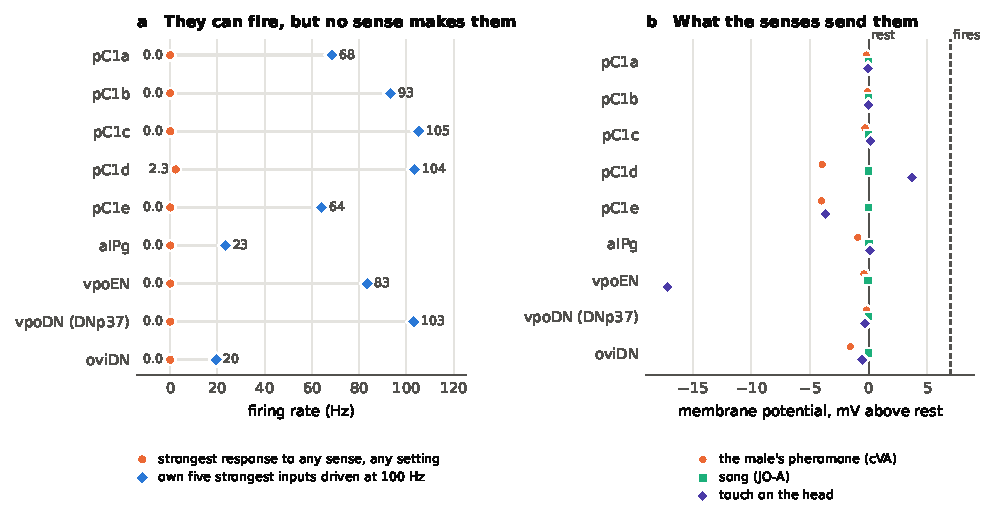
\includegraphics[width=\textwidth]{figures/fig_deciders.pdf}
\caption{The female's deciding neurons can fire, and the senses tell them no. \textbf{a}, the strongest rate each type of decider reaches to any sense in any setting (26 senses and combinations, synapse strengths 0.7--1.4, stimuli up to 300\,Hz, 14 versions of the model; 3 seeds each), against its rate when its own five strongest input types are driven at 100\,Hz. \textbf{b}, how full each decider's bucket gets under three senses at the published strength: its voltage in millivolts above rest (mean over its neurons and 3 seeds). A neuron fires at 7. Song here is steady firing of the ear's JO-A neurons.}
\label{fig:deciders}
\end{figure}

The model cannot start walking by itself either, though that is the most ordinary thing a fly does. In a clean box with nothing to smell but each other, two simulated females stood still for more than two minutes of brain time. Their eyes and noses fired, but not one descending neuron did. Part of this is the model's design: a model neuron has no activity of its own. Part is my smell-centre change, because under the published one the other fly's body odour sets them going (\Cref{sec:arena}). A real fly put in an empty dish soon walks about \citep{martin2004portrait}.

Most smells cause the opposite problem. A few seconds of the male's pheromone, a food odour or carbon dioxide leave about two thousand neurons firing on their own, the steering neurons among them. Twenty seconds after the smell had gone, when I stopped watching, they showed no sign of fading. I call this the self-sustaining state. Largely the same neurons fire whatever the smell. Touch, sound, sugar and the other fly's body odour alone leave nothing behind. The male's pheromone does the same in the male brain, and in the published models of both sexes the state takes in about eight thousand neurons. The state runs through the smell centre's excitatory local neurons. Turn them down to a tenth and it goes. Remove every connection from the brain back onto its own sensory neurons and it stays, so what keeps it going is in the brain itself \note{5}. In real flies the smell centre calms down soon after a smell ends \citep{wilson2004transformation}. The model's neurons never tire and its synapses never run down, so a loop of excitation, once lit, has nothing to put it out. But at a tenth most smells barely get through: only two of my ten test smells then set off more than a few dozen mushroom-body cells. So whether my version of the model keeps firing after a smell depends on how strong those local neurons really are, which nobody has measured.

Whichever rule I used to turn the transmitter guesses into ``go'' and ``stop'', the fly never steered clearly towards food. In my version, a food odour on one antenna turns her away. At gain 1.4 it still does in 11 of the 12 cases I tried. At 0.7 there is no turn to read, so like the backing this fails the synapse-strength test \note{5}.

% ══════════════════════════════════════════════════════════════════════════════
\section{What One State Adds}
\label{sec:states}

Keep the female's two virgin neurons firing and her acceptance neurons wake up \note{6}. Waking the acceptance neuron pC1a is no surprise, since the two virgin neurons supply nearly half its excitatory input. The signal also carries on one connection further, at every synapse strength I tried, to the yes neuron that opens her genital plate. Twenty random pairs of neurons with the same output strength (about as many synapses out) wake nothing. Nor do the virgin neurons in a rewired brain. This is half of the pathway traced in real flies \citep{wang2021neural}. A real virgin's yes neuron also needs the male's song, which reaches it through the song relay. In the model the relay stays silent even with song, and her deciders fire just as fast with or without the male's pheromone or song, so she says yes to nobody in particular. In the male I switched on the courtship neurons themselves, his deciders. They send his song command to the wing with nobody there to sing to, as they do in a real male on his own \citep{vonphilipsborn2011neuronal}. Twenty matched random sets of neurons do not, and nor do the courtship neurons in a rewired brain.

Keeping the hunger and fullness neurons firing, by contrast, changes no more than keeping an unrelated group firing. Partly that was bound to happen, since these neurons work mostly through neuropeptides, which the model lacks. In the female, the insulin (IPC) and DH44 neurons also have only about ten output synapses each. Her NPF, SIFa and AstA neurons have hundreds or thousands, but their paths to the feeding neurons are at most about a sixtieth as strong as sugar's, and two of the groups count as inhibitory here. So the states that work in this model are those whose neurons it treats as plain wires onto the deciders. That includes the virgin neurons, even though they are predicted to release serotonin, which acts as a neuromodulator in real flies.

The model also gets two things wrong. No state starts egg-laying. And at the model's standard settings a mated female (here, the brain with its virgin neurons left off) extends her ovipositor no more than a virgin, where a real one extends it more. Driving the virgin neurons three times as fast, or making every synapse 40 per cent stronger, makes the virgin's ovipositor neuron fire about a tenth less than the mated female's, which is the real direction.

% ══════════════════════════════════════════════════════════════════════════════
\section{What Learning Adds}
\label{sec:memory}

In the female model at its published strength, sugar and bitter tastes do not reach the dopamine teacher neurons. In real flies they do \citep{liu2012subset}, partly through octopamine, a neuromodulator whose chemical action the model lacks \citep{burke2012layered}. So I supplied the teaching signal myself whenever the fly tasted sugar, much as experimenters switch neurons on with light \note{7}, and the memory formed. After three pairings the smell that came with sugar reached the output neurons at about a tenth of its old strength, close to the lowest my rule allows. A second smell, given without sugar, kept about two-thirds. A teaching signal given just before the smell, or long after it, taught nothing. In one Minecraft run, on flowers that tasted of sugar, a weaker memory formed. In the male, whose map does not split sugar from bitter, taste as a whole does reach the punishment teachers. A smell paired with that taste then reaches the output neurons in those teachers' part of the mushroom body at half its old strength or less, with no help from me.

The fly did nothing with the memory. Where a before-and-after comparison exists, its walking and turning changed about as much as without the teaching signal. The route is there: driven hard, the memory's output neurons can turn the steering neurons on or off. But a smell drives them only weakly and reaches the steering neurons by other paths, so even silencing them barely changes what the legs receive. The memory is written in a notebook that is almost never opened. It could be opened more often if the neurons that the output neurons talk to sat closer to firing, as a fly's chemistry might keep them. With those neurons pushed to fire a few times a second, silencing the output neurons moved the left steering neurons by 3 to 7 spikes a second, against about 1 without the push. A memory can only quiet the output neurons, so silencing them is the most it could do, and I have not yet run a trained fly this way.

% ══════════════════════════════════════════════════════════════════════════════
\section{Two Flies in a Box}
\label{sec:arena}

The most entertaining results came from putting two flies in a box thirteen blocks across (\Cref{fig:arena}; \Cref{tab:arena}; Note~8). Every fly that walked in any box did so in the self-sustaining state, so the question is whether anything the flies sense steers them on top of it. Under the published smell centre the other fly's body odour starts the state. In that model the state drives the left steering neuron about nine times harder than the right, so two females circled to the left and never met. With my change, and a faint smell from flower patches that an earlier run had left by the wall, the females walked and bumped into each other by chance. Then they stayed together, because touch turned down their steering neurons. Real flies that bump into each other tend to move off \citep{ramdya2015mechanosensory}. These two stood pressed together for up to half a minute, extending their ovipositors at each other. A male and a female met far less often, and each meeting ended within seconds with the male walking backwards. In a properly cleaned box nothing moved, except that the male's pheromone set the female walking while he stood almost still until she touched him.

To get everyone moving I added a faint random input to every neuron, about one spike every five seconds, which I call the hum. Within a second or so it tips the brain into the self-sustaining state. On the hum, females met and stayed together, and males met females and backed out. On the bench, the touch of such a meeting drives his backing neurons most of the way on its own \note{4}. The male's song command never rose above the level the hum alone gives it, and neither did anyone's aggression neurons, except that a virgin female's reached about one spike a second on contact. Last, I ran two of the boxes again, three pairings in all, with new brain seeds and both flies let loose at the same moment, where before one had gone a few seconds ahead. The results held: two females on the hum met in every trial and on average spent almost half the time together, and a male and a female met briefly before he backed out. Then I switched off the females' sense of touch, which also took away their feel of the walls. They still met in every trial, but they no longer froze on contact, and the longest meeting fell from 16 seconds to under 4 (\Cref{tab:arena}; Note~8). So it is touch, through the freeze, that holds them together.

I measured whether a fly steers towards its partner before they first touch. In no box did it by more than a whisker, apart from the published model's steady left turn \note{9}. I first found a faint lean of the female towards the male, 24 recordings against 9. It came from her steady turn to the right and a male who happened to sit mostly on her right: with her own turning subtracted, 15 recordings lean towards him and 20 away. My flies are blind, and real males use sight to follow a female \citep{ribeiro2018visual}, so the box tests only whether the senses the flies have give them a reason to approach. A female whose virgin neurons I kept firing, on the hum with a male, makes the same point. Her yes neuron fired whether he was near or far, and her body logged nearly a hundred ``yes'' signals a minute, yet she did not steer towards him. Real virgins do not seek the male out either, but they slow down when he courts and open their genital plates when he sings \citep{bussell2014abdominal,wang2021neural}. Mine did neither in answer to him, apart from the stop that any touch causes.

\begin{figure}[tbp]
\centering
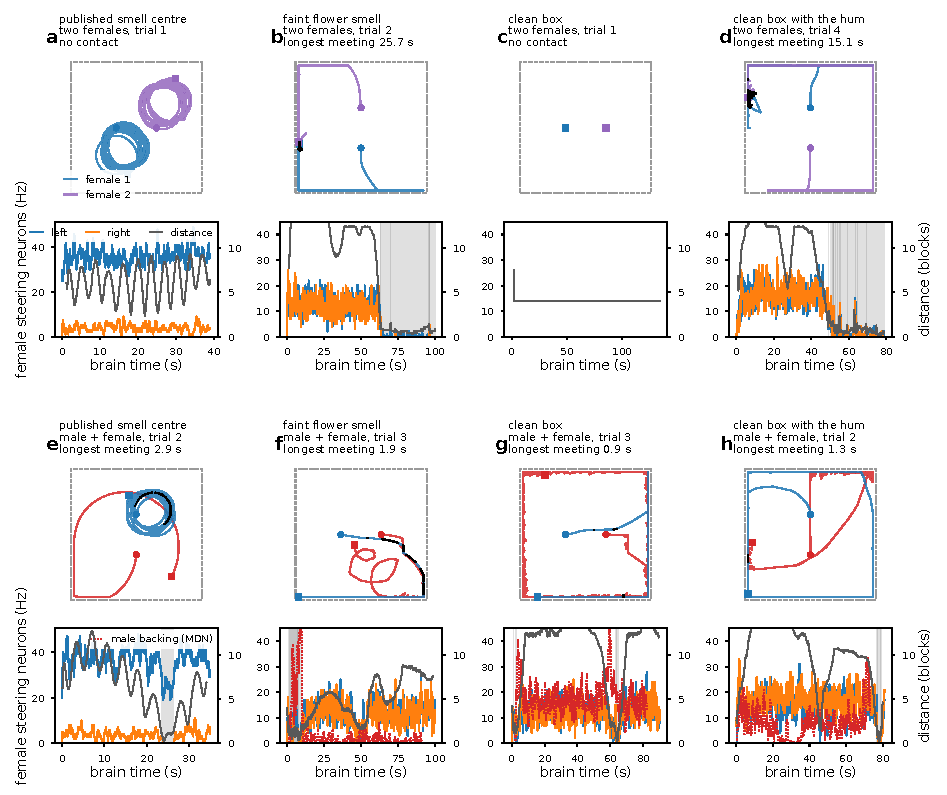
\includegraphics[width=\textwidth]{figures/fig3_print_encounters.pdf}
\caption{Two flies in a box, one trial for each box and pairing. \textbf{a--d}, two females; \textbf{e--h}, a male and a female, under the published smell centre (\textbf{a}, \textbf{e}), with my change and a faint flower smell at the wall (\textbf{b}, \textbf{f}), in a clean box (\textbf{c}, \textbf{g}) and in a clean box with the hum (\textbf{d}, \textbf{h}). Top: the paths walked (circle = start, square = end, black dots = contact, dashed = walls). Bottom: the female's left and right steering neurons, the distance between the flies (grey line), the male's backing neurons (red dotted) and contact (grey bands). Each panel shows the box's longest meeting (\textbf{a} and \textbf{c} had none), leaving out the two trials that began in contact because of the launch delay (Note 8).}
\label{fig:arena}
\end{figure}

% ══════════════════════════════════════════════════════════════════════════════
\section{Trying to Break It}
\label{sec:breaking}

I tried to break the results in three ways \note{10}. First, I re-ran the whole bench study from scratch, and all 124 result files it rewrote matched the previous run to the digit. Second, I had copies of the AI assistant check every sentence of a draft of this paper against the result files, and a further copy tried to argue away each problem that touched a main conclusion. Of 65 problems, 55 turned out to be real and 10 partly real. Most were wording that said more than the numbers do. A few were findings that did not survive, and the sections above say which. Third, I ran 60 new tests aimed at the claims (\Cref{tab:breaking}). For most I wrote the pass mark down before the run, and where a testing program repeats one of the paper's runs, I first made it reproduce the paper's result files to the digit.

\begin{table}[tbp]
\centering
\small
\renewcommand{\arraystretch}{1.12}
\begin{tabularx}{\textwidth}{@{}>{\RaggedRight}p{3.9cm}>{\RaggedRight}X>{\RaggedRight\arraybackslash}p{3.3cm}@{}}
\toprule
\textbf{Claim} & \textbf{How I tried to break it} & \textbf{What happened} \\
\midrule
The deciders are silent & every sense at gains 0.7--1.4 and at 200--300\,Hz, in all 14 model versions; their own inputs driven directly; the voltage and input of every decider; the inhibitory inputs silenced or flipped & holds in the female (at most 2--3\,Hz), not in the male, where cVA fires 1--14 of 148 courtship neurons (up to 30\,Hz), more with touch; mostly inhibition; with six guessed signs flipped the aggression deciders and song relay fire, the acceptance neurons still do not \\
The virgin state wakes them & gains 0.7--1.4; state rates 10--100\,Hz; 10 seeds; the hum; 20 random look-alike pairs; rewired brains & holds, but only half the real pathway \\
The courtship neurons send song & 20 random look-alike sets; the hum; one rewired brain & holds \\
Hunger does no more than an unrelated group & 10 seeds; the hum, in both sexes; added to the virgin state & holds (a 7\,Hz shift at 30\,Hz and 5 seeds shrank to 3\,Hz at 10 seeds; larger ones on the hum matched unrelated groups) \\
Reflexes are in the wiring & finer gains; stimulus rates 10--300\,Hz; a stricter rewiring & 2 hold throughout; 3 have a weak spot \\
The touched female freezes & weak connections removed (under 2 to 5 synapses); partial and one-sided touch; 5\,s of touch; other senses in place of touch & specific, but needs a strong touch and weak connections \\
The male backs away & gains; touch at 10--300\,Hz; what he smells; her touch, taste or smell removed & fails the gain test; touch gives most of it \\
The memory is learned & training in the wrong order; the teacher alone; other smells; longer training; two new seeds; a faster learning rule & holds \\
The memory is not used & its output neurons driven at up to 100\,Hz; a bypass of the smell route; the neurons they talk to kept close to firing & a route exists but is hardly used; with those neurons kept close to firing, silencing the output moves the steering neurons 3--7\,Hz \\
The model matches Shiu et al.'s & Shiu et al.'s code (in Brian2) on both versions of the model; time steps (the simulation's ticks) of 0.1--0.5\,ms; 3, 6 and 8 processor threads; new seeds & exact in full precision; smell runs drift apart; rates rise about 8\,\% at 0.5\,ms, because two timings round to the coarser tick \\
The model rests without input & smells, sugar, touch and sound for 3--10\,s, then silence; the smell centre's excitatory neurons turned down; the brain's connections onto its sensory neurons removed & fails after most smells; needs the smell centre's excitatory neurons \\
Nobody approaches & her own turning subtracted; his position shifted in time; each start counted once; new seeds & holds; the lean was not real \\
Touch keeps two females together & new seeds; their touch (of walls and of each other) switched off & holds (longest meeting 16\,s, under 4\,s without touch; no freeze on contact) \\
\bottomrule
\end{tabularx}
\caption{The tests aimed at each claim and what happened to it. Details in the notes and in \texttt{experiments/results\_edge/}.}
\label{tab:breaking}
\end{table}

% ══════════════════════════════════════════════════════════════════════════════
\section{Counterarguments}
\label{sec:counterarguments}

\subsection{``A Model This Simple Cannot Tell You Anything About a Real Fly''}

It cannot tell you what a real fly does. That needs a real fly. It can tell you what a complete wiring diagram contains when run with some of the simplest rules anyone has proposed. Some of what the model does, real flies do with the same neurons (feeding, grooming, the escape neuron, the first half of the virgin pathway). Some has no counterpart in a fly, such as a male backing away from a female he touches or tastes. So what the model does is a candidate for experiments, and what it cannot do points to candidates for what is missing.

\subsection{``Of Course a Model Without Hormones Cannot Be Hungry''}

Some of the negative results are unsurprising, and I have said which (\Cref{sec:states}). But the virgin state is partly chemical in real flies too, since sex peptide, a chemical the male passes on in mating, ends it \citep{feng2014ascending}. The state still works in the model because its last steps run on synapses. And a memory written entirely in synapses still hardly ever reaches the legs.

\subsection{``You Adjusted the Smell Centre Until It Did What You Wanted''}

I chose a quarter from four settings before I had written a test for it. Before a finer sweep I fixed a test in advance: different smells must set off largely different cells in the mushroom body. A quarter was still the mildest cut that passed it. At the published synapse strength, results that do not involve smell come out much the same either way, except that sugar sometimes sets off the published smell centre. The result that hangs most on the setting is the self-sustaining state, and with it the walking in the box. The state is larger without my change and absent at a tenth.

\subsection{``Five Trials Per Box Is Not Enough''}

For rates and proportions it is modest, and the notes give the spreads. Most of the arena claims are about presence or absence (no song command above what the hum alone gives, no steering towards the partner). Those need fewer trials, though what counts is the number of trials and not the number of moments recorded. Fifteen more trials with new seeds gave the same answers (\Cref{tab:arena}).

% ══════════════════════════════════════════════════════════════════════════════
\section{What Would Prove Me Wrong}
\label{sec:refutation}

Four things would defeat my argument.

\begin{enumerate}[leftmargin=*]
  \item A more faithful version of the same diagram would use measured transmitters or synapse strengths, or add electrical synapses. If one woke the female's acceptance neurons from the senses alone, or the male's courtship neurons from a female's touch or taste, the silence I found would belong to the simplified model. In real flies one pathway both excites and inhibits the male's courtship neurons \citep{clowney2015multimodal,kallman2015excitation}, a balance that a model in which every synapse pours the same cupful cannot set.
  \item Any reflex that disappears once predicted transmitters are replaced by measured ones along its path is not in the wiring. Of the behaviours here the freeze is the most fragile, since it rides on weak connections.
  \item If adding neuromodulation to the model, for example neuropeptide release from the hunger neurons, still left hunger doing nothing, then what is missing is not chemistry.
  \item If the self-sustaining state went out once the model's neurons were given a way to tire, that state would belong to the simplified neuron rather than to the wiring.
\end{enumerate}

The model also makes two predictions. A strong touch over most of a walking fly's head should quiet its steering neurons DNa01 and DNa02 while its ovipositor neuron fires, and a touch to a tenth of the bristles should not. And the fast drive from the head bristles to the ovipositor neuron should differ little between virgin and mated females. In the model it differs by about a tenth at most, so a large extra ovipositor extension in mated females would come from something slower, such as neuromodulation.

% ══════════════════════════════════════════════════════════════════════════════
\section{Limitations}
\label{sec:limitations}

The model has no neuromodulation, no electrical synapses, no development, no fatigue and no running down of synapses. Every neuron has the same leak and threshold, and the female model has no nerve cord. Dopamine, serotonin and octopamine, which act as neuromodulators in real flies, count here as ordinary excitatory synapses, and every neuron gets one sign, guessed by the classifier unless its transmitter is known. Sound arrives as steady firing, without the rhythm of real song. The male map does not split sugar from bitter taste, and I turned the male's synapses down so that his neurons get as much input on average as hers, which is a guess. Real flies start walking with descending neurons such as DNp09 \citep{bidaye2020two}, which answer no sense in this model, so I read walking from the steering neurons. The flies are blind. The arena is small, and one wiring diagram per sex cannot show how much real flies differ. Note 11 lists my other choices.

% ══════════════════════════════════════════════════════════════════════════════
\section{Conclusion}
\label{sec:conclusion}

A fruit fly's complete wiring diagram, set running with some of the simplest rules anyone has proposed, knows how to eat and how to hold out an ovipositor when touched. Less reliably, it knows how to jump at a loud noise and how to groom. Nobody had to put any of that in. It does not know what it wants. Its deciding neurons hear mostly ``no'' or nothing from the senses, and the female's acceptance neurons wake only once I keep her virgin neurons firing from outside. In a real fly that switch is set partly by chemistry, which is where I would look next, and where I would point anyone paying for the next map.

Two copies of my fly brain, mapped synapse by synapse, once stood in a clean white box for two minutes with only their eyes and noses working, like parked cars with the keys left in.

\bigskip
\noindent\emph{Solomon Shalom Lijo is an independent researcher.} \href{mailto:solomon@getromy.app}{\emph{solomon@getromy.app}}.

% ══════════════════════════════════════════════════════════════════════════════
\clearpage
\section*{Notes}
\small

\begin{enumerate}[leftmargin=*, label=\arabic*., itemsep=4pt]

\item \emph{The model.} Leaky integrate-and-fire neurons with Shiu et al.'s constants ($v_\text{rest}=v_\text{reset}=-52$\,mV, threshold $-45$\,mV, $\tau_m=20$\,ms, $\tau_\text{syn}=5$\,ms, refractory period 2.2\,ms, delay 1.8\,ms, $w=0.275$\,mV per synapse $\times$ sign; sensory drive by Poisson kicks of 68.75\,mV; $dt=0.2$\,ms; single precision). With no input the brain never spikes. Female: FlyWire v783 as Shiu et al.'s connection table (15{,}090{,}883 connections, 54.5\,M synapses; one sign per neuron from its predicted transmitter, \citealt{eckstein2024neurotransmitter}; annotations from \citealt{schlegel2024whole}). Male: MaleCNS v1.0 \citep{berg2026sexual}, 164{,}439 neurons and 25.6\,M connections, every synapse scaled by 0.542 so that a brain neuron's mean input matches the female's (a guess, which the gain test also tests). \emph{Against Brian2} \citep{stimberg2019brian}, a transcription of Shiu et al.'s code (sugar at 100\,Hz for 1\,s, 3 seeds, $dt=0.1$\,ms): in double precision every spike falls on the same step. In single precision two seeds differ, each first at one neuron just short of threshold ($1.3\times10^{-5}$ and $2.8\times10^{-6}$\,mV). In one only that spike moves. In the other the difference spreads: 4{,}563 of Brian2's 23{,}512 spikes fall on another step or neuron, though the totals differ by under 1\,\% (23{,}689 against 23{,}512; per-neuron correlation 0.9999). Runs that switch on the self-sustaining state (Note~5) drift further apart, because small differences grow in it (cVA at 0.1 against 0.2\,ms: 0.1--24\,\%; correlation 0.9974). \emph{Time step} (10 seeds of 1\,s; a rate counts if either run gives at least 1\,Hz, and two means differ if they are two standard errors or more apart): at 0.1\,ms, 6 of 116 rates differ from 0.2\,ms, about as many as chance gives. At 0.5\,ms the refractory period rounds to 2.0\,ms and a spike takes 2.5\,ms to arrive instead of 2.0 (an arrival acts one step after the rounded delay), and rates rise by a median 8\,\% (at most 7\,Hz). Run at 0.1\,ms with those two values, rates match 0.5\,ms (5 of 115 differ, none by more than 2.05\,Hz), so the rounding accounts for the rise (I did not separate the two values). The deciders stay at 0 and the freeze index at 0.69--0.97 throughout. \emph{Threads}: 3 and 8 threads change the one-second probe by at most 0.4\,Hz in any five-seed mean, and the same thread count reproduces every file to the digit.

\item \emph{The three tests.} (i) Every synapse at 0.7, 1.0 and 1.4 times its published strength; in the female, smell responses need 1.0 or more. (ii) Degree-preserving rewiring \citep{maslov2002specificity} in two forms. With any target allowed (99.8--99.9\,\% of connections move; 3 female and 2 male brains, one of each re-run with 35--42 inputs), the descending neurons together fire at most 0.2\,Hz even under touch (8.1\,Hz intact). In each brain every readout averages 0--2.2\,Hz over seeds, except the punishment dopamine neurons at up to 3.3\,Hz under whole-head touch and four groups of 2--4 neurons at up to 6.4\,Hz (MDN, DNp13, DNp09 and aSP22). With each connection moved only within its target's broad class (94\,\% move; female, my model, 2 brains), sugar, wind, JO-B and smells no longer reach their targets, the virgin neurons wake nobody and within 0.8\,s no smell starts the self-sustaining state; JO-A $\rightarrow$ giant fibre survives at 5.2 and 7.5\,Hz (10.6 intact), and head touch drives the giant fibre at 56--92\,Hz, MDN at 21--40 and the steering neurons at 29--66\,Hz, with DNp13 below the descending-neuron average. (iii) A sensitivity table: stimulus 50 and 150\,Hz, time step 0.1 and 0.5\,ms, the first-version numerics, three ways of turning the transmitter predictions into signs, four smell-centre settings, a second connection table and a $\geq 5$-synapse threshold (14 female conditions, 13 male). The three sign rules all use the same classifier's predictions, so none tests a wrong guess; Note~5 does that for the deciders.

\item \emph{The smell centre.} Published model: one glomerulus at 100\,Hz makes 81\,\% of the 685 projection neurons and 65\,\% of the 5{,}177 Kenyon cells fire, the same cells for every odour (overlap 0.99). My two changes: the known transmitter wherever one is recorded (11{,}010 neurons, 8{,}359 of them photoreceptors), and the output of the 150 antennal-lobe local neurons that the sign rule makes excitatory (71 predicted cholinergic; 38 serotonergic, 16 GABAergic, 12 dopaminergic, 11 glutamatergic and 2 octopaminergic) $\times$\,0.25. I chose 0.25 on 15--16 September from four settings (1, 0.5, 0.25, 0.1) without a numeric criterion. Before a finer sweep on 27 September I fixed one: two different odours overlap by at most 0.25 in the Kenyon cells, one odour with itself by at least twice that, and odours drive on average at most 35\,\% of glomeruli. Of nine settings from 1 to 0.1, 0.25 is the largest that meets it (0.16 between odours, 0.78 within, 18\,\% of glomeruli); 0.3 narrowly fails (0.27) and 0.2 passes. At 0.15 and 0.1 only DM1 and the food blend that contains it drive more than 0.5\,\% of Kenyon cells (the others at most 0.4\,\%). At 0.25 each odour drives 0--5\,\% of Kenyon cells, as in real flies \citep{honegger2011cellular}. At gain 1.0 every female readout that does not involve smell is identical at $\times$0.25 and $\times$1 and within 4\,Hz of the published model, except that sugar sets off the published smell centre in 1 of 5 female runs and 3 of 5 male runs. At gain 1.4 touch and taste do it more often (touch $\rightarrow$ DNp13 19 against 42\,Hz).

\item \emph{The reflexes} (female unless stated; gains 0.7 / 1.0 / 1.4; 100\,Hz stimulus). \emph{Sugar} $\rightarrow$ MN9 33 / 76 / 94\,Hz, and 64--95\,Hz in 13 of 14 conditions (371\,Hz under the first-version numerics). \emph{Bitter}: with Shiu et al.'s 29 sugar neurons MN9 fires 55\,Hz, and 3.3\,Hz with bitter added (4.4\,$\pm$\,3.7 over 10 seeds); it keeps 3--13\,\% of its rate in 12 conditions, and 9, 25 and 39\,\% at gains 1.0, 1.2 and 1.4. \emph{Head bristles} $\rightarrow$ DNp13 28 / 35 / 42\,Hz and 28--51\,Hz in all 14 conditions, graded with the touch (5--35\,Hz at 10--100\,Hz; 20\,Hz from a quarter of the bristles); a touch on one side drives only that side's DNp13. \emph{Sound} (JO-A) $\rightarrow$ giant fibre 5 / 11 / 16\,Hz (10 seeds), 18--28\,Hz at 150--300\,Hz, but 1.6\,Hz at 50\,Hz. \emph{Antenna} (Shiu et al.'s 69 JO-CE neurons) $\rightarrow$ aBN1 0.5 / 13 / 32\,Hz, and 0.6\,Hz under the $\geq5$-synapse threshold. \emph{The freeze}: a food odour drives the steering neurons DNa01/02 at 20/12\,Hz, and all 1{,}417 head and eye bristles at 100\,Hz bring them to 6.8/3.2 (freeze index 0.69\,$\pm$\,0.06); under cVA they go from 9/8 to 0/1.2 (0.93). The index is 0.69--0.93 from gain 1.0 to 2.0 (at 0.7 smells barely drive the DNa), 0.31--0.98 in every condition but the $\geq5$-synapse threshold, and deepens from 0.78 to 0.86 over 5\,s. Other senses in place of touch give $-$0.12 to 0.13. It needs a strong touch: all bristles at 10--100\,Hz give $-$0.25 to 0.69, a tenth of them at 200\,Hz $-$0.44, and one side alone 0.16--0.69. Removing connections of fewer than 2, 3 and 5 synapses takes it to 0.59, 0.37 and 0.00. DNp09 answers no sense (at most 0.7\,Hz). \emph{Male}: his 162 pooled labellar taste neurons leave his MN9 at 0\,Hz at gains up to 1.0. cVA $\rightarrow$ DNp13 7.8 / 30 / 26\,Hz, and every other odour gives DNp13 0. Leg taste (ppk23/25) $\rightarrow$ wing motor neurons 20 / 22 / 11\,Hz (not specific: wind 14, cVA 13) and MDN 0 / 27 / 1.8\,Hz, with P1 at 0. Head bristles $\rightarrow$ MDN 0 / 10.7 / 11.8\,Hz. By touch rate (gain 1.0; 3 seeds of 0.6\,s), MDN is 0 at 10--50\,Hz and 11.5, 27.5, 50.4 and 66.5\,Hz at 100, 150, 200 and 300\,Hz, and with cVA added 8.2, 23.1, 40.3, 54.2 and 67.6\,Hz at 50 to 300\,Hz. A bench stand-in for a meeting in the box (Or47b at 100\,Hz, ppk25 at 150\,Hz and his 819 head and eye bristle neurons at 200\,Hz) gives MDN 58.6\,$\pm$\,2.4\,Hz: 58.1 without the smell, 55.0 without the taste and 27.2\,$\pm$\,5.1 without the touch ($p=0.003$). At gains 0.7 and 1.4 touch was tested only at 100\,Hz.

\item \emph{Deciders, walking and the self-sustaining state.} \emph{Deciders}: pC1a--c, pC1e, vpoEN, vpoDN (DNp37) and oviDN fire 0.0\,Hz in every neuron to each of 26 inputs and combinations at gains 0.7--1.4, at 200 and 300\,Hz, in all 14 conditions and to touch at 10--300\,Hz (3 seeds); pC1d reaches at most 2.5\,Hz and aIPg one spike in a run, and on the hum every decider stays at its 0.1--0.5\,Hz floor. At gain 2.0, outside the test range, pC1d/e average up to 4.1\,Hz (5 seeds). Male P1/pC1 (148 neurons typed pC1\_, 86 of them P1 proper, annotated pMP-e/pMP4) average at most 0.5\,Hz at gains up to 1.0 (5 seeds), but single neurons fire (a mean over 3 seeds of 1\,s above 2\,Hz). With cVA one fires at gain 1.0 (pC1\_3c, 6.3\,Hz) and 14 at 1.4 (up to 30\,Hz); with cVA and touch, five at 1.0 (up to 18\,Hz) and 17 at 1.4 (up to 36\,Hz); with touch alone none at 1.0 and one at 1.4. Of the 22 that ever pass 2\,Hz, 21 are pMP-e/pMP4 (P1) types and one is pC1\_11a. At 0.7 all are silent. This fails the pass mark set in advance (no single neuron above about 5\,Hz). The song command pIP10 answers only inputs that include cVA (3.3\,$\pm$\,1.6\,Hz at gain 1.0, 7.3--7.5\,Hz at 1.4; any other input at most 0.5\,Hz), and touch added to cVA cuts it (0 at 1.0, 1.2--1.7\,Hz at 1.4). \emph{Positive control}: driving each decider's five strongest presynaptic cell types at 100\,Hz makes pC1a fire at 68\,Hz, pC1b 93, pC1c 105, pC1d 104, pC1e 64, aIPg 23, vpoEN 83, vpoDN 103 and oviDN 20 (the two oviDNb neurons are not among the targets of those types and have no positive control). \emph{What reaches them} (voltage above rest, mean over neurons and 3 seeds; firing needs 7\,mV): touch lifts pC1d to +3.7\,mV (peak 5.3; 6.4 at gain 1.4), cVA pushes pC1d and pC1e to $-$4\,mV, touch holds vpoEN at $-$17\,mV, song moves pC1a--e by less than 0.05\,mV, pC1a and pC1b receive at most 280 synapse$\cdot$Hz of excitation from any sense, and pC1e and oviDN receive 8--74 times more inhibition than excitation. Every decider is one to three connections from every sense, and 60 of 102 sense--decider pairs are net inhibitory (by path weight: each connection's signed share of its target's input, multiplied along routes of one to four connections). In the male, P1, pIP10, aIPg and vpoEN/DN are also one to three connections from every sense (32 of 68 pairs net inhibitory). cVA's path to P1 is net excitatory, about half of it through LH008m (aSP-f), and leg taste reaches P1 mainly through ascending AN09B017 neurons (vAB3), which the model makes inhibitory. These weights predict firing poorly: cVA's path to pIP10 is net inhibitory, yet cVA is the one input pIP10 answers. The inhibition onto pC1d, pC1e and vpoEN passes mostly through six cell types predicted to be GABAergic (AOTU064, AVLP531, PS088, CB0584, WED104, PVLP021; prediction confidence 0.74--0.92, none measured); pC1e's also through CB0626, which I did not test. Silencing their output, with or without the measured-GABA oviIN, leaves every decider at 0.0\,Hz at gain 1.0, and pC1d at most 1.2\,Hz at 1.4 (3.5 in one seed). Flipping it to excitatory (3 seeds) lets cVA drive pC1d at 18 and pC1e at 7\,Hz and touch drive vpoEN at 39\,Hz (DNp37 3\,Hz) at gain 1.0; at 1.4, cVA drives pC1d at 27, pC1e at 19 and oviDN at 10\,Hz, and touch drives vpoEN at 56, DNp37 at 25 and oviDN at 10\,Hz. pC1a and pC1b stay at 0 and pC1c at most 0.3\,Hz.
\emph{Steering} (steering neurons on the odour's side minus the other side, averaged over a left and a right presentation so that a fixed turn cancels): under my signs a food odour on one antenna turns her away by 1--7\,Hz at every strength from 25 to 150\,Hz (four food odours, 10 seeds; 218 of 240 values negative), read within the self-sustaining state. At gain 1.4 (50--150\,Hz, 5 seeds) the mean turn is away by 2--9\,Hz in 11 of 12 odour and strength pairs, less consistently (51 of 60 values negative; ester at 50\,Hz gives +1.4\,$\pm$\,2.8\,Hz). At gain 0.7 there is no turn to read: every smell I ran there leaves the steering neurons at 0, except food at up to 1.5\,Hz in single runs (vinegar, ester and sweet were not run at 0.7). cVA on one antenna does not reliably turn her towards it at gain 1.0 or 1.4. Under the published signs (with my smell-centre change) a fixed left turn of 8--29\,Hz masks a pull of up to 3.8\,Hz towards food. \emph{Clean box}: two females, every descending neuron at 0.00 in 10 recordings of 135\,$\pm$\,6\,s, while about 8\,\% of neurons fired (photoreceptors, and each other's body odour and CO$_2$). \emph{Self-sustaining state} (3\,s of input, then 20\,s of nothing; 2 seeds): cVA, a food odour or CO$_2$ at 25--100\,Hz leaves 1{,}915--2{,}067 neurons firing in 17 of 18 runs, with the steering neurons at 13--22\,Hz, MN9, DNp13 and every decider at 0, and no decay over 20\,s. Or47b (the other fly's body odour) and sound leave nothing. After 10\,s of input, sound, touch and sugar leave nothing either, but Or47b at 90\,Hz with CO$_2$ at 3\,Hz starts the state within 2\,s (2 seeds). Largely the same neurons fire whichever smell starts it (overlap 0.86--0.91): 1{,}720--1{,}850 central neurons, among them antennal-lobe local and projection neurons, lateral-horn and Kenyon cells, and 125--150 descending neurons. It grows with synaptic strength (with a food odour, about 700 neurons at gain 0.7, not reaching the steering neurons, and 4{,}300--5{,}100 at 1.4) and with the published smell centre (8{,}300 neurons, 3{,}364 of them Kenyon cells; steering neurons 36\,Hz left and 4\,Hz right; there Or47b starts it too). The hum starts it within about a second at 0.2\,Hz. In the male, cVA leaves 1{,}950--2{,}100 neurons and a food odour about 920 (steering neurons at most 2.5\,Hz), and his published model about 7{,}900; touch and his contact pheromone leave nothing. With the excitatory local neurons at $\times$0.1 or $\times$0 the state does not start (a loop of 75--78 neurons that reaches no descending neuron keeps firing in half the runs); with every synapse onto a sensory neuron removed it does (1{,}846--1{,}913 neurons; 7{,}700 in the published model).
In arena recordings the share of active neurons is 8.0\,\% for the still females of the clean box and 9.0--10.3\,\% for every fly that walked (13.6\,\% under the published smell centre).

\item \emph{Internal states} (a group of the fly's own state neurons driven at 30\,Hz). SAG (2 neurons) $\rightarrow$ pC1a 21.2\,$\pm$\,3.9\,Hz, pC1b and pC1c 18.9, and vpoDN (DNp37) 17.2\,$\pm$\,3.4\,Hz, all from 0 (10 seeds; vpoEN stays silent, also with song); with touch, pC1d 14\,Hz. SAG supplies 387 of pC1a's 824 excitatory input synapses. By gain 0.7 / 1.0 / 1.4: pC1a 12 / 21 / 30\,Hz. Driving SAG at 10 to 100\,Hz (it fires at 11--84\,Hz; 3--10 seeds), pC1a rises steadily from 5.0 to 61.3\,Hz and pC1b/c from 4.8 to 56.4\,Hz; pC1a fires at 0.65--0.78 of SAG's own rate from 20\,Hz up and 0.45 at 10\,Hz (the pass mark set in advance was 0.6--0.8). Twenty random pairs of ascending neurons matched to SAG's output strength wake none of these neurons, and neither does SAG in any rewired brain. Adding NPF, IPC, AstA or DH44 to SAG (10 seeds; SIFa not tested) moves pC1a, pC1b/c and DNp37 by $-$3.1 to +1.2\,Hz (Welch $p\geq0.07$), mostly because SAG itself then fires a little slower; the pass mark set in advance (within 2 SEM of SAG alone) holds in 121--127 of 128 decider cells. P1/pC1 (the 148 neurons of Note~5) $\rightarrow$ pIP10 50.4\,$\pm$\,1.2 and TN1 8.2\,$\pm$\,0.5\,Hz (at most 3.8 and 1.8 without the state); twenty random sets of 148 central neurons matched for output strength give pIP10 at most 0.8\,Hz and TN1 0, and in a rewired male brain (Note~2) P1 gives pIP10 0 and the song motor neurons 0 (49.8 and 27.2 intact). (The song motor neurons also reach 21\,Hz on contact pheromone alone, so only pIP10 and TN1 are specific to the state.) Output synapses per neuron in the female: IPC 9, DH44 12, NPF 622, SIFa 468, AstA 11{,}936, SAG 684. NPF, SIFa and AstA are two connections from MN9, as sugar is, but their strongest path weighs at most $2.4\times10^{-5}$ against sugar's $1.7\times10^{-3}$ (to the feeding motor neurons $1.6\times10^{-5}$ against $9.5\times10^{-4}$). In the female, IPC, DH44, SIFa and AstA recruit no other neuron at rest at any state rate from 10 to 100\,Hz; NPF recruits none up to 30\,Hz and 1--3 at 60--100\,Hz, and SAG 35--103 at 30\,Hz. With sugar the five move MN9 by $-$0.4 to +3.5\,Hz and unrelated states by $-$0.2 to +3.5 at 30\,Hz (10 seeds; ANOVA over ten states $p=0.43$; NPF's +6.8\,Hz in the first 5 seeds fell to +3.2), but by +1.2 to +6.8 against $-$6.2 to +5.2 at 100\,Hz (5 seeds; $p=0.001$); on the hum no hunger shift can be told apart from those of unrelated states (the largest, on the erratic MN9, are within 2.1\,Hz of the unrelated state given the same noise). In the male on the hum (5 seeds), P1 still drives pIP10 to 44.2\,$\pm$\,3.3 and TN1 to 6.9\,$\pm$\,1.0\,Hz, against 0.2\,Hz with no state and at most 3.4 and 1.4\,Hz under any other state and input. His hunger and fullness states do no more than unrelated ones (the few larger shifts are on MN9 and MDN, whose rates jump from seed to seed on the hum; all Welch $p\geq0.085$), though with his MN9 silent to taste the test says little about feeding.
Touch $\rightarrow$ DNp13 is 36.0\,$\pm$\,0.8\,Hz without a state and 36.1\,$\pm$\,0.7 with SAG. At gain 1.4 SAG lowers it from 41.9 to 37.9\,Hz (5 seeds; $p=0.04$). With the state neurons driven at 100\,Hz, SAG lowers it from 35.6\,$\pm$\,1.0 to 32.3\,$\pm$\,1.4\,Hz (5 seeds; Welch $p=0.004$, which meets the rule set in advance for qualifying this miss) and pC1a--c to 28.3\,$\pm$\,1.4\,Hz ($p=2\times10^{-5}$), while no other state lowers it by more than 0.9\,Hz. At 10--60\,Hz neither moves touch alone by more than 1.5\,Hz ($p\geq0.12$); with cVA added, at 60\,Hz, they lower it by 2.2 and 4.2\,Hz ($p=0.04$ and 0.05). oviDN is 0 under every state, at every gain and state rate.

\item \emph{Learning.} Dopamine-gated weakening of Kenyon cell $\rightarrow$ output-neuron synapses (rate 0.3\,s$^{-1}$, floor 10\,\%, 1\,s eligibility trace; the constants are mine). In the female, sugar, bitter and touch drive 0.0\,Hz in every dopamine neuron at gain 1.0 and 50--150\,Hz; bitter reaches the punishment set at gain 1.4 (2.4\,Hz) or at 200--300\,Hz; in the male, the pooled labellar taste neurons drive the 16 PPL1 neurons at 11.7\,Hz (0.0 at gain 0.7). So the teaching signal drives the identified reward (PAM) or punishment (PPL1) neurons at 50\,Hz while the fly tastes sugar or bitter. Offline, three 10-s pairings with 5-s rests, both odour orders (a shortened version of the design of \citealt{tully1985classical}): the paired odour keeps 0.10--0.11 of its drive (about the floor) and the other 0.59--0.70; learning index (the other's kept drive minus the paired one's) 0.55\,$\pm$\,0.03 ($n=6$), 0.03 without a teaching signal ($n=4$, $-$0.01 to +0.08). Teaching signal just before the odour, or 5\,s after it: $-$0.08 to +0.05. Teaching signal alone: both odours keep 0.85--0.95. Index for other pairs: floral/vinegar (no glomerulus shared) 0.72 and 0.63, ester/sweet (four of six shared) 0.43 and 0.15. Six pairings instead of three: 0.47 and 0.53. Two held-out seeds (3 and 4, both orders) give 0.52--0.60, 0.42--0.67 above their matched runs without a teaching signal. At a learning rate of 1\,s$^{-1}$ instead of 0.3 (seed 0) the index falls to 0.48 and 0.44, below all ten runs at 0.3, because the other odour keeps less (0.57 and 0.54, against 0.70 and 0.59); about three-quarters of that extra loss also happens without a teaching signal.
Punishment: 0.35 with vinegar paired and 0.08 with ester paired, but without a teaching signal the same compartment already gives +0.28 and $-$0.24 (vinegar lowers its own input there), so pairing adds 0.07 and 0.31. Male (seed 0): 0.80 and 0.77 with the reward and punishment sets driven, each read in its own compartment. With his 162 pooled labellar taste neurons at 100\,Hz in place of the teaching signal, the reward compartment gives 0.01 and 0.04 (PAM 0.0\,Hz), but the punishment compartment gives 0.42 and 0.61 (the paired odour keeps 0.48 and 0.31 of its drive there), because taste drives the punishment set at 8.9--12.6\,Hz through the wiring; so his punishment result has no control without a teaching signal.
In the world (one run each): the sugar-paired smell kept 0.29 of its drive and the other 0.66 (index 0.37); the punishment run's 0.29 is matched by 0.31 in a run with no bitter at all, so it is not learning. \emph{Expression}: no descending neuron changes consistently with the pairing (the steering neurons shift by up to 7\,Hz between tests, and by 6.5\,Hz without a teaching signal). Driving the 20 punishment output neurons at 20--100\,Hz moves 24--27 descending types, the left steering neurons to 19--23\,Hz from 0; one type (MBON14) alone at 50\,Hz gives 18\,Hz. Driving the 12 reward output neurons at 50--100\,Hz during a smell turns down 14--18 descending types. But a smell drives the output neurons at only 0.5--12\,Hz, and silencing either set moves the steering neurons by at most 1.3\,Hz and no descending type by more than 4.5\,Hz. With the output neurons' non-descending targets kept close to firing instead (50 extra inputs to each, calibrated as set in advance so that the targets fire 1--10\,Hz without a smell; 3 seeds), silencing the punishment set lowers the left steering neurons by 5.0--7.3\,Hz under vinegar on both antennae (lower in all 15 paired runs) and single descending types by up to 8.5\,Hz, and silencing the reward set, the one sugar trains, raises them by 3.2--4.2\,Hz (single types by up to 7.8\,Hz). Both fail the pass mark set in advance (every change below 5\,Hz). With vinegar on one antenna the left--right difference hardly moves ($-$0.8\,Hz), and with 3 seeds the gap to the unpushed brain is suggestive ($p=0.13$--0.19).

\item \emph{The box.} 13 $\times$ 13 blocks, white walls, no food. The flies start 4 blocks apart, facing each other (trials 1 and 3) or away from each other (2 and 4), or 5.7 blocks apart on a diagonal (5), in the same order in every series. Each series before 27 September used brain seeds 1--5, the same seed for both flies of a pair. Trials ran 300\,s (180\,s in the first series; 600\,s in the replication's hum and virgin series). Contact means within 1.3 blocks, the range of the touch sense; touching another fly, a wall or being hit drives all 1{,}417 head and eye bristle neurons of both sides (819 in the male) at 200\,Hz. The second fly was let loose about 3--5\,s after the first; in two faint-smell trials the first fly walked onto the second's starting point in that time, so the pair began in contact. They are left out of \Cref{tab:arena} (without them the longest meeting is 25.7\,s, and 31.1\,s in the replication). The hum is an independent Poisson input to every neuron of both brains at 0.2\,Hz; on it, away from the walls and the other fly, DNp13 fires under 0.5\,Hz (the 5.3\,Hz far from the other fly in \Cref{tab:arena} comes from touching the walls, which drives it at about 20\,Hz), females lunge twice a minute, and the male's body plays 20--25 song acts a minute (60--130 in contact, from the leg-taste reflex of Note 4, with the song command pIP10 at 0.2\,Hz). The replication's clean male--female series ran on a laptop so loaded that the body's slow-down to brain time failed (a median 0.8\,s of wall time per 50\,ms of brain time), so that series is not comparable with the original. The series of 27 September used new brain seeds (101--105) and let both flies loose together, each body waiting for the other before its brain starts (launch gap at most 0.23\,s; no trial began in contact); its hum series ran 600\,s and its clean-box series 300\,s, and in one hum series every head and eye bristle input of both females was switched off. The female brain has no leg-taste neurons, so this removes every sense of contact, with the walls as well as the other fly: in contact these females walked 0.51 of the time against 0.04 with touch, with steering neurons at 9.7/16.4 against 0.8/0.3\,Hz. The first trial of that series stalled at its start (a tenth of its brain steps took more than 0.8\,s of wall time); leaving it out changes no number in the text.

\item \emph{Approach.} The turn-toward index is the turn command times the side the partner is on, averaged over the moments within 6 blocks before a first contact (turn commands average about 0.25 in size). It is $-$0.02 to +0.04 in every series of my model (the four of 27 September included), and $-$0.19 (two females) and +0.08 (male and female) under the published smell centre, whose flies turn left whatever is where. Pooled over the male--female recordings of my model before 27 September, the raw index is positive in 24 of the 35 that turn at all, negative in 9 and zero in 2 (sign test $p=0.014$). But she turns right in 30 of the 35 and the male sits mostly on her right in 27. After subtracting each female's own mean turn when he is 6 or more blocks away, 15 recordings lean towards him and 20 away ($p=0.50$; pooled index +0.009, under a twentieth of a typical turn). Subtracting her mean over all moments gives 17 and 18, comparing her turning with him on the left and on the right within a recording gives 6 and 6, and shifting his position in time against her turning gives $P=0.15$. The recordings are not independent, since every series before 27 September used the same five seeds and starts: counted once per start, the raw lean is 5 of 5 ($p=0.06$) and the corrected one 3 towards and 2 away. Female pairs: 13 and 9 raw, 11 and 11 corrected. The series of 27 September give 7 and 3 raw and 6 and 4 corrected (male and female) and 9 and 11 raw and 8 and 12 corrected (female pairs). The virgin female's index is $-$0.005 and +0.040 in the two series; her DNp37 fires 15.8--16.6\,Hz far from the male, near him and in contact alike.

\item \emph{Trying to break it.} \emph{Re-run}: \texttt{reproduce.sh}'s 15 offline groups, one at a time under a queue that paused work if free memory ran low (6 threads; 4\,h\,23\,min; peak 2.6\,GB; no pause needed). All 124 rewritten result files are identical to the digit to the previous run. \emph{Audit}: seven copies of the assistant mapped each claim to its evidence; nine re-derived 65 problems from the files (55 confirmed, 10 partly, none refuted), and a further copy tried to refute each problem that touched a main conclusion. \emph{New tests}: 56 steps on the bench and 4 series in the box (20 trials); steps listed in \texttt{experiments/edge/steps\_20260927.tsv}, pass marks in \texttt{experiments/edge/design\_plan.md} (written before the runs; the decider controls, the self-sustaining-state probes, the sign-flip test, the held-out learning seeds, the naming of the male neurons and three of the four box series were added after it and had none; the fourth, two females on the hum, met its mark of three genuine meetings in five, one of them 10\,s or more), results in \texttt{experiments/results\_edge/} and \texttt{experiments/edge/analysis\_A.md} and \texttt{analysis\_B.md}. The test programs that repeat runs of the paper were first made to reproduce its result files to the digit (1{,}620 cells of the sensory probe, 728 of the sensitivity table, the conditioning and expression files byte for byte). Five new seeds reproduce every one-second number of Notes 4 and 5 within seed noise (4 of 115 rates differ by more than two standard errors). Each edge-case test ran once, with the seeds given above.

\item \emph{What is the fly's and what is mine.} The fly's: every neuron and connection, its synapse count, its sign, its side and the identities of the neurons. Mine: the simulation constants (Shiu et al.'s), the male's scale, the smell-centre changes, which blocks smell of what, how far a smell carries (16 blocks), the stimulus rates (100\,Hz on the bench, at most 150\,Hz in the body, 200\,Hz for touch), how firing becomes movement (walking is $1-e^{-r/10\,\text{Hz}}$ of the mean rate of DNa01/02 and turning $\tanh$ of their left--right difference over 40\,Hz), two body reflexes that stand in for the nerve cord (stepping up a one-block ledge, floating in water), the learning constants and teaching signal, the hum and the synchronised start. The eyes fire with the light, but the signal dies in the optic lobe.

\end{enumerate}

\begin{table}[h]
\centering
\footnotesize
\setlength{\tabcolsep}{3.2pt}
\renewcommand{\arraystretch}{1.12}
\resizebox{\textwidth}{!}{%
\begin{tabular}{@{}lcccccccc@{}}
\toprule
Pair & Trials with & Contact & Longest & Walking & Steering neurons, & Ovipositor neuron, & Toward & Male MDN \\
 & contact & (\% of time) & meeting (s) & (share) & far $\rightarrow$ contact (L/R, Hz) & far $\rightarrow$ contact (Hz) & index & on contact (Hz) \\
\midrule
\multicolumn{9}{@{}l}{\emph{Published smell centre, no smell in the box (14 Sep)}} \\
two females & 0/5 & 0.0 $\pm$ 0.0 & -- & 0.71 & 36.1/4.2 $\rightarrow$ -- & 0.0 $\rightarrow$ -- & $-$0.191 & -- \\
male + female & 4/5 & 3.6 $\pm$ 3.5 & 2.9 & 0.71 & 37.1/4.0 $\rightarrow$ 20.9/0.1 & 0.0 $\rightarrow$ 16.5 & +0.079 & 0 \\
\multicolumn{9}{@{}l}{\emph{Changed smell centre, faint flower smell at the wall (17 Sep)}} \\
two females & 2/3 & 20.4 $\pm$ 16.8 & 25.7 & 0.39 & 12.8/12.9 $\rightarrow$ 0.4/0.0 & 6.1 $\rightarrow$ 32.8 & +0.011 & -- \\
male + female & 1/5 & 1.2 $\pm$ 2.6 & 1.9 & 0.47 & 12.4/12.4 $\rightarrow$ 2.7/1.2 & 5.7 $\rightarrow$ 33.0 & +0.014 & 40 \\
\multicolumn{9}{@{}l}{\emph{Changed smell centre, clean box (18 Sep)}} \\
two females & 0/5 & 0.0 $\pm$ 0.0 & -- & 0.00 & 0.0/0.0 $\rightarrow$ -- & 0.0 $\rightarrow$ -- & +0.000 & -- \\
male + female & 2/5 & 0.5 $\pm$ 0.9 & 0.9 & 0.48 & 12.7/12.6 $\rightarrow$ 0.0/0.3 & 5.1 $\rightarrow$ 31.6 & $-$0.021 & 48 \\
\multicolumn{9}{@{}l}{\emph{Clean box with the 0.2\,Hz hum (18--19 Sep)}} \\
two females & 3/5 & 11.2 $\pm$ 14.9 & 15.1 & 0.51 & 15.5/16.3 $\rightarrow$ 1.2/1.2 & 5.3 $\rightarrow$ 30.8 & +0.002 & -- \\
male + female & 4/5 & 1.3 $\pm$ 1.1 & 1.3 & 0.55 & 15.2/16.1 $\rightarrow$ 2.0/1.8 & 5.1 $\rightarrow$ 30.6 & +0.033 & 29 \\
\multicolumn{9}{@{}l}{\emph{Clean box with the hum, virgin female (24 Sep)}} \\
male + female & 5/5 & 3.6 $\pm$ 3.2 & 1.7 & 0.52 & 13.9/15.9 $\rightarrow$ 0.3/1.4 & 4.1 $\rightarrow$ 31.7 & $-$0.005 & 30 \\
\midrule
\multicolumn{9}{@{}l}{\emph{Again: Changed smell centre, clean box (25--26 Sep)}} \\
two females & 0/5 & 0.0 $\pm$ 0.0 & -- & 0.00 & 0.0/0.0 $\rightarrow$ -- & 0.0 $\rightarrow$ -- & +0.000 & -- \\
male + female$^\dagger$ & 2/5 & 1.8 $\pm$ 3.7 & 0.6 & 0.53 & 14.1/15.5 $\rightarrow$ 5.0/5.3 & 1.4 $\rightarrow$ 30.3 & +0.011 & 37 \\
\multicolumn{9}{@{}l}{\emph{Again: Clean box with the 0.2\,Hz hum (25--26 Sep)}} \\
two females & 5/5 & 59.1 $\pm$ 15.8 & 31.1 & 0.25 & 15.6/17.0 $\rightarrow$ 0.9/0.4 & 4.5 $\rightarrow$ 30.9 & +0.028 & -- \\
male + female & 3/5 & 1.5 $\pm$ 1.5 & 2.5 & 0.59 & 16.5/17.8 $\rightarrow$ 0.8/1.0 & 3.8 $\rightarrow$ 30.6 & +0.012 & 31 \\
\multicolumn{9}{@{}l}{\emph{Again: Clean box with the hum, virgin female (25--26 Sep)}} \\
male + female & 5/5 & 6.3 $\pm$ 7.2 & 4.5 & 0.52 & 14.5/16.9 $\rightarrow$ 0.3/0.9 & 3.5 $\rightarrow$ 31.7 & +0.040 & 30 \\
\midrule
\multicolumn{9}{@{}l}{\emph{New seeds, flies started together: clean box with the hum (27 Sep)}} \\
two females & 5/5 & 46.1 $\pm$ 27.4 & 15.8 & 0.30 & 14.0/14.9 $\rightarrow$ 0.8/0.3 & 7.1 $\rightarrow$ 31.0 & $-$0.018 & -- \\
male + female & 5/5 & 3.7 $\pm$ 2.7 & 6.2 & 0.51 & 14.2/14.9 $\rightarrow$ 1.6/1.3 & 6.8 $\rightarrow$ 32.0 & +0.014 & 30 \\
\multicolumn{9}{@{}l}{\emph{The same, with the females' touch switched off (27 Sep)}} \\
two females & 5/5 & 5.6 $\pm$ 3.0 & 3.6 & 0.66 & 18.9/21.9 $\rightarrow$ 9.7/16.4 & 0.2 $\rightarrow$ 0.3 & +0.030 & -- \\
\multicolumn{9}{@{}l}{\emph{New seeds, flies started together: clean box (27 Sep)}} \\
male + female & 2/5 & 1.0 $\pm$ 1.7 & 2.1 & 0.42 & 11.3/10.7 $\rightarrow$ 0.3/0.6 & 7.8 $\rightarrow$ 30.6 & +0.003 & 44 \\
\bottomrule
\end{tabular}}
\caption{Every box, series by series, with the replication (``Again'') at the bottom. Female values are means over the female fly-logs (both flies in a female pair, the female in a male--female pair), five trials per row, $\pm$ the standard deviation across fly-logs; contact means within 1.3 blocks, the range of the touch sense; far means more than 3.5 blocks away. Walking is the share of time the fly spent walking. Far values include moments against a wall, which the body feels as touch, so the walls, not the hum, set the ovipositor neuron's far values (about 20\,Hz against a wall, under 0.5\,Hz away from walls and flies, 0.2\,Hz with touch switched off). Trials ran 300\,s (180\,s in the 14 Sep series; 600\,s in the replication's hum and virgin series, because other work on the laptop had slowed the brains). The toward index is the turn command times the side the other fly is on, over the moments within six blocks before a first contact (positive = towards). The faint-smell female pairs lost two of their five trials, which began in contact because the first fly was let loose a few seconds before the second (Note 8). $^\dagger$The laptop was so loaded during this series that the body's slow-down to brain time failed, so it cannot be compared with the original. The last block repeats three of the series above (two females, and a male and a female, on the hum; a male and a female in the clean box) with new brain seeds and both flies started together, in trials of 600\,s (300\,s in the clean box), and adds a fourth on the hum in which the females' touch, of the walls as well as of each other, was switched off. Written by \texttt{experiments/replication\_stats.py}.}
\label{tab:arena}
\end{table}


\paragraph{Data and code.} All code and result files are at \url{https://github.com/solomonshalom/flycraft}. The release archive written by \texttt{reproduce.sh archive}, which adds every arena log, will be deposited at Zenodo. The connectomes are public: FlyWire v783 \citep{dorkenwald2024neuronal,schlegel2024whole}, used as Shiu et al.'s table (\url{https://github.com/philshiu/Drosophila_brain_model}), and MaleCNS v1.0 \citep{berg2026sexual}.

\paragraph{Funding.} The author is an independent researcher. This work received no external funding.

\normalsize

% ══════════════════════════════════════════════════════════════════════════════
% References
% ══════════════════════════════════════════════════════════════════════════════
\begin{thebibliography}{99}
\bibliographystyle{apalike}

\bibitem[Aso et~al.(2014)]{aso2014neuronal}
Aso, Y., Hattori, D., Yu, Y., Johnston, R.~M., Iyer, N.~A., Ngo, T.-T.~B., et~al. (2014). The neuronal architecture of the mushroom body provides a logic for associative learning. \emph{eLife}, 3, e04577. \url{https://doi.org/10.7554/eLife.04577}

\bibitem[Bargmann \& Marder(2013)]{bargmann2013connectome}
Bargmann, C.~I., \& Marder, E. (2013). From the connectome to brain function. \emph{Nature Methods}, 10, 483--490. \url{https://doi.org/10.1038/nmeth.2451}

\bibitem[Berg et~al.(2026)]{berg2026sexual}
Berg, S., Beckett, I.~R., Costa, M., Schlegel, P., Januszewski, M., Marin, E.~C., et~al. (2026). Sexual dimorphism in the complete \emph{Drosophila} male central nervous system connectome. \emph{Cell}, 189, 5504--5526.e15. \url{https://doi.org/10.1016/j.cell.2026.08.015}

\bibitem[Bidaye et~al.(2014)]{bidaye2014neuronal}
Bidaye, S.~S., Machacek, C., Wu, Y., \& Dickson, B.~J. (2014). Neuronal control of \emph{Drosophila} walking direction. \emph{Science}, 344, 97--101. \url{https://doi.org/10.1126/science.1249964}

\bibitem[Bidaye et~al.(2020)]{bidaye2020two}
Bidaye, S.~S., Laturney, M., Chang, A.~K., Liu, Y., Bockem\"{u}hl, T., B\"{u}schges, A., et~al. (2020). Two brain pathways initiate distinct forward walking programs in \emph{Drosophila}. \emph{Neuron}, 108, 469--485.e8. \url{https://doi.org/10.1016/j.neuron.2020.07.032}

\bibitem[Burke et~al.(2012)]{burke2012layered}
Burke, C.~J., Huetteroth, W., Owald, D., Perisse, E., Krashes, M.~J., Das, G., et~al. (2012). Layered reward signalling through octopamine and dopamine in \emph{Drosophila}. \emph{Nature}, 492, 433--437. \url{https://doi.org/10.1038/nature11614}

\bibitem[Bussell et~al.(2014)]{bussell2014abdominal}
Bussell, J.~J., Yapici, N., Zhang, S.~X., Dickson, B.~J., \& Vosshall, L.~B. (2014). Abdominal-B neurons control \emph{Drosophila} virgin female receptivity. \emph{Current Biology}, 24, 1584--1595. \url{https://doi.org/10.1016/j.cub.2014.06.011}

\bibitem[Capra(2022)]{capra2022metaphysics}
Capra, B. (2022). The metaphysics of farts. \emph{Think}, 21(61), 39--43. \url{https://doi.org/10.1017/S1477175621000452}

\bibitem[Clowney et~al.(2015)]{clowney2015multimodal}
Clowney, E.~J., Iguchi, S., Bussell, J.~J., Scheer, E., \& Ruta, V. (2015). Multimodal chemosensory circuits controlling male courtship in \emph{Drosophila}. \emph{Neuron}, 87, 1036--1049. \url{https://doi.org/10.1016/j.neuron.2015.07.025}

\bibitem[Deutsch et~al.(2020)]{deutsch2020neural}
Deutsch, D., Pacheco, D., Encarnacion-Rivera, L., Pereira, T., Fathy, R., Clemens, J., et~al. (2020). The neural basis for a persistent internal state in \emph{Drosophila} females. \emph{eLife}, 9, e59502. \url{https://doi.org/10.7554/eLife.59502}

\bibitem[Dorkenwald et~al.(2024)]{dorkenwald2024neuronal}
Dorkenwald, S., Matsliah, A., Sterling, A.~R., Schlegel, P., Yu, S.~C., McKellar, C.~E., et~al. (2024). Neuronal wiring diagram of an adult brain. \emph{Nature}, 634, 124--138. \url{https://doi.org/10.1038/s41586-024-07558-y}

\bibitem[Dudai et~al.(1976)]{dudai1976dunce}
Dudai, Y., Jan, Y.~N., Byers, D., Quinn, W.~G., \& Benzer, S. (1976). \emph{dunce}, a mutant of \emph{Drosophila} deficient in learning. \emph{Proceedings of the National Academy of Sciences USA}, 73, 1684--1688. \url{https://doi.org/10.1073/pnas.73.5.1684}

\bibitem[Eckstein et~al.(2024)]{eckstein2024neurotransmitter}
Eckstein, N., Bates, A.~S., Champion, A., Du, M., Yin, Y., Schlegel, P., et~al. (2024). Neurotransmitter classification from electron microscopy images at synaptic sites in \emph{Drosophila melanogaster}. \emph{Cell}, 187, 2574--2594.e23. \url{https://doi.org/10.1016/j.cell.2024.03.016}

\bibitem[Feng et~al.(2014)]{feng2014ascending}
Feng, K., Palfreyman, M.~T., H\"{a}semeyer, M., Talsma, A., \& Dickson, B.~J. (2014). Ascending SAG neurons control sexual receptivity of \emph{Drosophila} females. \emph{Neuron}, 83, 135--148. \url{https://doi.org/10.1016/j.neuron.2014.05.017}

\bibitem[Greenspan \& Ferveur(2000)]{greenspan2000courtship}
Greenspan, R.~J., \& Ferveur, J.~F. (2000). Courtship in \emph{Drosophila}. \emph{Annual Review of Genetics}, 34, 205--232. \url{https://doi.org/10.1146/annurev.genet.34.1.205}

\bibitem[Hampel et~al.(2015)]{hampel2015neural}
Hampel, S., Franconville, R., Simpson, J.~H., \& Seeds, A.~M. (2015). A neural command circuit for grooming movement control. \emph{eLife}, 4, e08758. \url{https://doi.org/10.7554/eLife.08758}

\bibitem[Honegger et~al.(2011)]{honegger2011cellular}
Honegger, K.~S., Campbell, R.~A.~A., \& Turner, G.~C. (2011). Cellular-resolution population imaging reveals robust sparse coding in the \emph{Drosophila} mushroom body. \emph{Journal of Neuroscience}, 31, 11772--11785. \url{https://doi.org/10.1523/JNEUROSCI.1099-11.2011}

\bibitem[Hoopfer et~al.(2015)]{hoopfer2015p1}
Hoopfer, E.~D., Jung, Y., Inagaki, H.~K., Rubin, G.~M., \& Anderson, D.~J. (2015). P1 interneurons promote a persistent internal state that enhances inter-male aggression in \emph{Drosophila}. \emph{eLife}, 4, e11346. \url{https://doi.org/10.7554/eLife.11346}

\bibitem[Kallman et~al.(2015)]{kallman2015excitation}
Kallman, B.~R., Kim, H., \& Scott, K. (2015). Excitation and inhibition onto central courtship neurons biases \emph{Drosophila} mate choice. \emph{eLife}, 4, e11188. \url{https://doi.org/10.7554/eLife.11188}

\bibitem[Kohatsu et~al.(2011)]{kohatsu2011female}
Kohatsu, S., Koganezawa, M., \& Yamamoto, D. (2011). Female contact activates male-specific interneurons that trigger stereotypic courtship behavior in \emph{Drosophila}. \emph{Neuron}, 69, 498--508. \url{https://doi.org/10.1016/j.neuron.2010.12.017}

\bibitem[Kurtovic et~al.(2007)]{kurtovic2007single}
Kurtovic, A., Widmer, A., \& Dickson, B.~J. (2007). A single class of olfactory neurons mediates behavioural responses to a \emph{Drosophila} sex pheromone. \emph{Nature}, 446, 542--546. \url{https://doi.org/10.1038/nature05672}

\bibitem[Lijo(2026a)]{lijo2026compound}
Lijo, S.~S. (2026a). The compound infeasibility thesis: A structural argument against single-axis approaches to AGI feasibility. \emph{Minds and Machines (forthcoming)}.

\bibitem[Lijo(2026c)]{lijo2026niche}
Lijo, S.~S. (2026c). In defense of niche benchmarks: Why the long tail of LLM evaluation matters. \emph{arXiv preprint}.

\bibitem[Lijo(2026b)]{lijo2026pifbench}
Lijo, S.~S. (2026b). PIF-Bench: Evaluating prospect intelligence fidelity in AI-assisted donor research. \emph{arXiv preprint}.

\bibitem[Lijo(2026e)]{lijo2026spirits}
Lijo, S.~S. (2026e). Testing the spirits: A Pentecostal reading of the AI sycophancy problem. \emph{arXiv preprint}.

\bibitem[Lijo(2026d)]{lijo2026tsb}
Lijo, S.~S. (2026d). TSB: A time-saved benchmark for AI systems. \emph{arXiv preprint}.

\bibitem[Liu et~al.(2012)]{liu2012subset}
Liu, C., Pla\c{c}ais, P.-Y., Yamagata, N., Pfeiffer, B.~D., Aso, Y., Friedrich, A.~B., et~al. (2012). A subset of dopamine neurons signals reward for odour memory in \emph{Drosophila}. \emph{Nature}, 488, 512--516. \url{https://doi.org/10.1038/nature11304}

\bibitem[Marder(2012)]{marder2012neuromodulation}
Marder, E. (2012). Neuromodulation of neuronal circuits: Back to the future. \emph{Neuron}, 76, 1--11. \url{https://doi.org/10.1016/j.neuron.2012.09.010}

\bibitem[Martin(2004)]{martin2004portrait}
Martin, J.~R. (2004). A portrait of locomotor behaviour in \emph{Drosophila} determined by a video-tracking paradigm. \emph{Behavioural Processes}, 67, 207--219. \url{https://doi.org/10.1016/j.beproc.2004.04.003}

\bibitem[Maslov \& Sneppen(2002)]{maslov2002specificity}
Maslov, S., \& Sneppen, K. (2002). Specificity and stability in topology of protein networks. \emph{Science}, 296, 910--913. \url{https://doi.org/10.1126/science.1065103}

\bibitem[Mezzera et~al.(2020)]{mezzera2020ovipositor}
Mezzera, C., Brotas, M., Gaspar, M., Pavlou, H.~J., Goodwin, S.~F., \& Vasconcelos, M.~L. (2020). Ovipositor extrusion promotes the transition from courtship to copulation and signals female acceptance in \emph{Drosophila melanogaster}. \emph{Current Biology}, 30, 3736--3748.e5. \url{https://doi.org/10.1016/j.cub.2020.06.071}

\bibitem[MICrONS Consortium(2025)]{microns2025functional}
MICrONS Consortium (2025). Functional connectomics spanning multiple areas of mouse visual cortex. \emph{Nature}, 640, 435--447. \url{https://doi.org/10.1038/s41586-025-08790-w}

\bibitem[Pool \& Scott(2014)]{pool2014feeding}
Pool, A.~H., \& Scott, K. (2014). Feeding regulation in \emph{Drosophila}. \emph{Current Opinion in Neurobiology}, 29, 57--63. \url{https://doi.org/10.1016/j.conb.2014.05.008}

\bibitem[Ramdya et~al.(2015)]{ramdya2015mechanosensory}
Ramdya, P., Lichocki, P., Cruchet, S., Frisch, L., Tse, W., Floreano, D., \& Benton, R. (2015). Mechanosensory interactions drive collective behaviour in \emph{Drosophila}. \emph{Nature}, 519, 233--236. \url{https://doi.org/10.1038/nature14024}

\bibitem[Rayshubskiy et~al.(2025)]{rayshubskiy2025neural}
Rayshubskiy, A., Holtz, S.~L., Bates, A.~S., Vanderbeck, Q.~X., Serratosa Capdevila, L., Rockwell, V., et~al. (2025). Neural circuit mechanisms for steering control in walking \emph{Drosophila}. \emph{eLife}, 13, RP102230. \url{https://doi.org/10.7554/eLife.102230}

\bibitem[Ribeiro et~al.(2018)]{ribeiro2018visual}
Ribeiro, I.~M.~A., Drews, M., Bahl, A., Machacek, C., Borst, A., \& Dickson, B.~J. (2018). Visual projection neurons mediating directed courtship in \emph{Drosophila}. \emph{Cell}, 174, 607--621.e18. \url{https://doi.org/10.1016/j.cell.2018.06.020}

\bibitem[Ryner et~al.(1996)]{ryner1996control}
Ryner, L.~C., Goodwin, S.~F., Castrillon, D.~H., Anand, A., Villella, A., Baker, B.~S., et~al. (1996). Control of male sexual behavior and sexual orientation in \emph{Drosophila} by the \emph{fruitless} gene. \emph{Cell}, 87, 1079--1089. \url{https://doi.org/10.1016/S0092-8674(00)81802-4}

\bibitem[Schlegel et~al.(2024)]{schlegel2024whole}
Schlegel, P., Yin, Y., Bates, A.~S., Dorkenwald, S., Eichler, K., Brooks, P., et~al. (2024). Whole-brain annotation and multi-connectome cell typing of \emph{Drosophila}. \emph{Nature}, 634, 139--152. \url{https://doi.org/10.1038/s41586-024-07686-5}

\bibitem[Schretter et~al.(2020)]{schretter2020cell}
Schretter, C.~E., Aso, Y., Robie, A.~A., Dreher, M., Dolan, M.~J., Chen, N., et~al. (2020). Cell types and neuronal circuitry underlying female aggression in \emph{Drosophila}. \emph{eLife}, 9, e58942. \url{https://doi.org/10.7554/eLife.58942}

\bibitem[Shiu et~al.(2024)]{shiu2024drosophila}
Shiu, P.~K., Sterne, G.~R., Spiller, N., Franconville, R., Sandoval, A., Zhou, J., et~al. (2024). A \emph{Drosophila} computational brain model reveals sensorimotor processing. \emph{Nature}, 634, 210--219. \url{https://doi.org/10.1038/s41586-024-07763-9}

\bibitem[Siegel \& Hall(1979)]{siegel1979conditioned}
Siegel, R.~W., \& Hall, J.~C. (1979). Conditioned responses in courtship behavior of normal and mutant \emph{Drosophila}. \emph{Proceedings of the National Academy of Sciences USA}, 76, 3430--3434. \url{https://doi.org/10.1073/pnas.76.7.3430}

\bibitem[Stimberg et~al.(2019)]{stimberg2019brian}
Stimberg, M., Brette, R., \& Goodman, D.~F.~M. (2019). Brian 2, an intuitive and efficient neural simulator. \emph{eLife}, 8, e47314. \url{https://doi.org/10.7554/eLife.47314}

\bibitem[Tully \& Quinn(1985)]{tully1985classical}
Tully, T., \& Quinn, W.~G. (1985). Classical conditioning and retention in normal and mutant \emph{Drosophila melanogaster}. \emph{Journal of Comparative Physiology A}, 157, 263--277. \url{https://doi.org/10.1007/BF01350033}

\bibitem[von Philipsborn et~al.(2011)]{vonphilipsborn2011neuronal}
von Philipsborn, A.~C., Liu, T., Yu, J.~Y., Masser, C., Bidaye, S.~S., \& Dickson, B.~J. (2011). Neuronal control of \emph{Drosophila} courtship song. \emph{Neuron}, 69, 509--522. \url{https://doi.org/10.1016/j.neuron.2011.01.011}

\bibitem[von Reyn et~al.(2014)]{vonreyn2014spike}
von Reyn, C.~R., Breads, P., Peek, M.~Y., Zheng, G.~Z., Williamson, W.~R., Yee, A.~L., et~al. (2014). A spike-timing mechanism for action selection. \emph{Nature Neuroscience}, 17, 962--970. \url{https://doi.org/10.1038/nn.3741}

\bibitem[Wang \& Anderson(2010)]{wang2010identification}
Wang, L., \& Anderson, D.~J. (2010). Identification of an aggression-promoting pheromone and its receptor neurons in \emph{Drosophila}. \emph{Nature}, 463, 227--231. \url{https://doi.org/10.1038/nature08678}

\bibitem[Wang et~al.(2020)]{wang2020neural}
Wang, F., Wang, K., Forknall, N., Patrick, C., Yang, T., Parekh, R., et~al. (2020). Neural circuitry linking mating and egg laying in \emph{Drosophila} females. \emph{Nature}, 579, 101--105. \url{https://doi.org/10.1038/s41586-020-2055-9}

\bibitem[Wang et~al.(2021)]{wang2021neural}
Wang, K., Wang, F., Forknall, N., Yang, T., Patrick, C., Parekh, R., et~al. (2021). Neural circuit mechanisms of sexual receptivity in \emph{Drosophila} females. \emph{Nature}, 589, 577--581. \url{https://doi.org/10.1038/s41586-020-2972-7}

\bibitem[White et~al.(1986)]{white1986structure}
White, J.~G., Southgate, E., Thomson, J.~N., \& Brenner, S. (1986). The structure of the nervous system of the nematode \emph{Caenorhabditis elegans}. \emph{Philosophical Transactions of the Royal Society of London B}, 314, 1--340. \url{https://doi.org/10.1098/rstb.1986.0056}

\bibitem[Wilson et~al.(2004)]{wilson2004transformation}
Wilson, R.~I., Turner, G.~C., \& Laurent, G. (2004). Transformation of olfactory representations in the \emph{Drosophila} antennal lobe. \emph{Science}, 303, 366--370. \url{https://doi.org/10.1126/science.1090782}

\bibitem[Yaksi \& Wilson(2010)]{yaksi2010electrical}
Yaksi, E., \& Wilson, R.~I. (2010). Electrical coupling between olfactory glomeruli. \emph{Neuron}, 67, 1034--1047. \url{https://doi.org/10.1016/j.neuron.2010.08.041}

\bibitem[Zhou et~al.(2014)]{zhou2014central}
Zhou, C., Pan, Y., Robinett, C.~C., Meissner, G.~W., \& Baker, B.~S. (2014). Central brain neurons expressing doublesex regulate female receptivity in \emph{Drosophila}. \emph{Neuron}, 83, 149--163. \url{https://doi.org/10.1016/j.neuron.2014.05.038}

\end{thebibliography}

\end{document}

